\begin{sepframe}{OOP}{A quick reminder}
\end{sepframe}

\begin{frame}[fragile,c]
    \frametitle{Composition and inheritance}
    \framesubtitle{Map}

    \makebox[\linewidth]{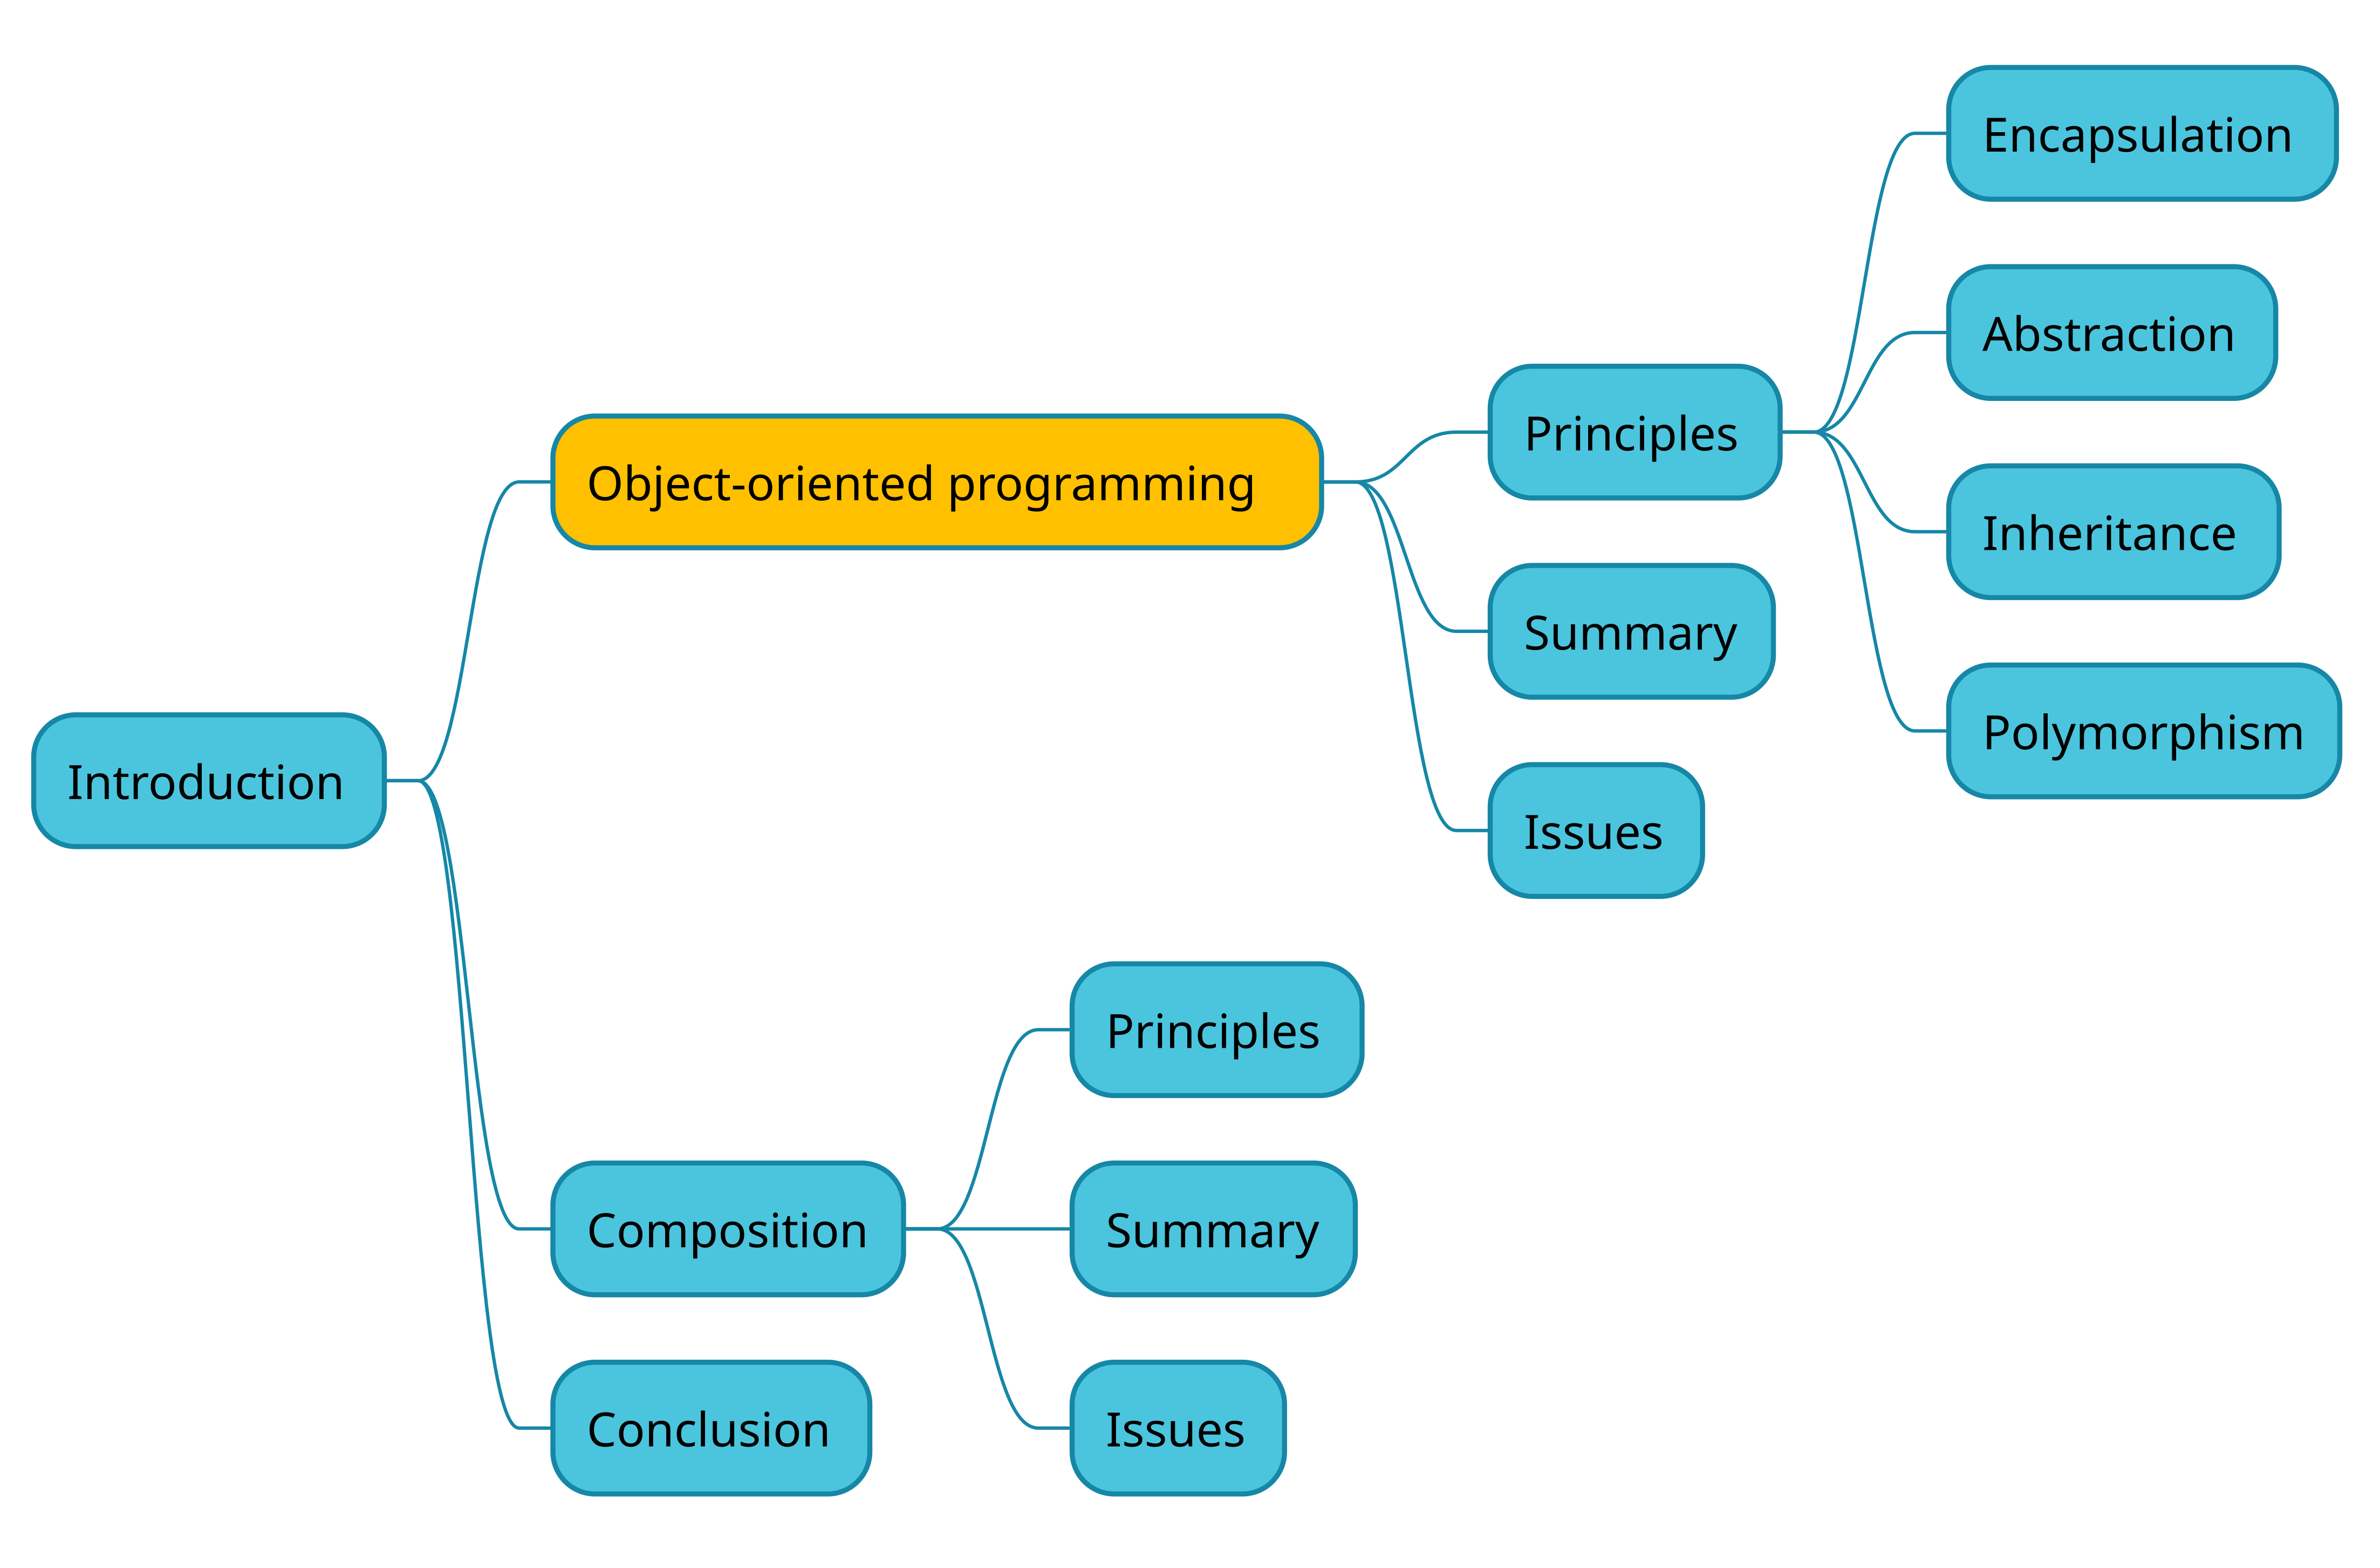
\includegraphics[width=\paperwidth]{src/session--composition-and-inheritance/resources/summary-oop-intro.png}}
\end{frame}

\begin{frame}
    \begin{quote}
        \textbf{O}bject-\textbf{O}riented \textbf{P}rogramming (\textbf{\textit{OOP}}) is more than just classes and objects.\\\pause

        It's a whole programming paradigm based around objects that contain data fields and methods.\\

        \pause

        It is \textbf{essential} to understand this.\\

        \pause

        Using classes to organize a bunch of unrelated methods together is \textbf{not} OOP per se.\\

        \vspace{10 mm}

        \hfill Junade Ali, Mastering PHP Design Patterns

        \hfill ISBN-13: \href{https://www.amazon.com/Mastering-PHP-Design-Patterns-Junade/dp/1785887130}{978-1785887130}
    \end{quote}
\end{frame}

\begin{frame}[c]
    \begin{center}
        \Huge What \pause makes \pause code \pause \textbf{OOP} ?
    \end{center}
\end{frame}

\begin{frame}[c]
    \begin{center}
        \Huge The principles!
    \end{center}
\end{frame}

\begin{frame}[fragile,c]
    \frametitle{Composition and inheritance}
    \framesubtitle{Map}

    \makebox[\linewidth]{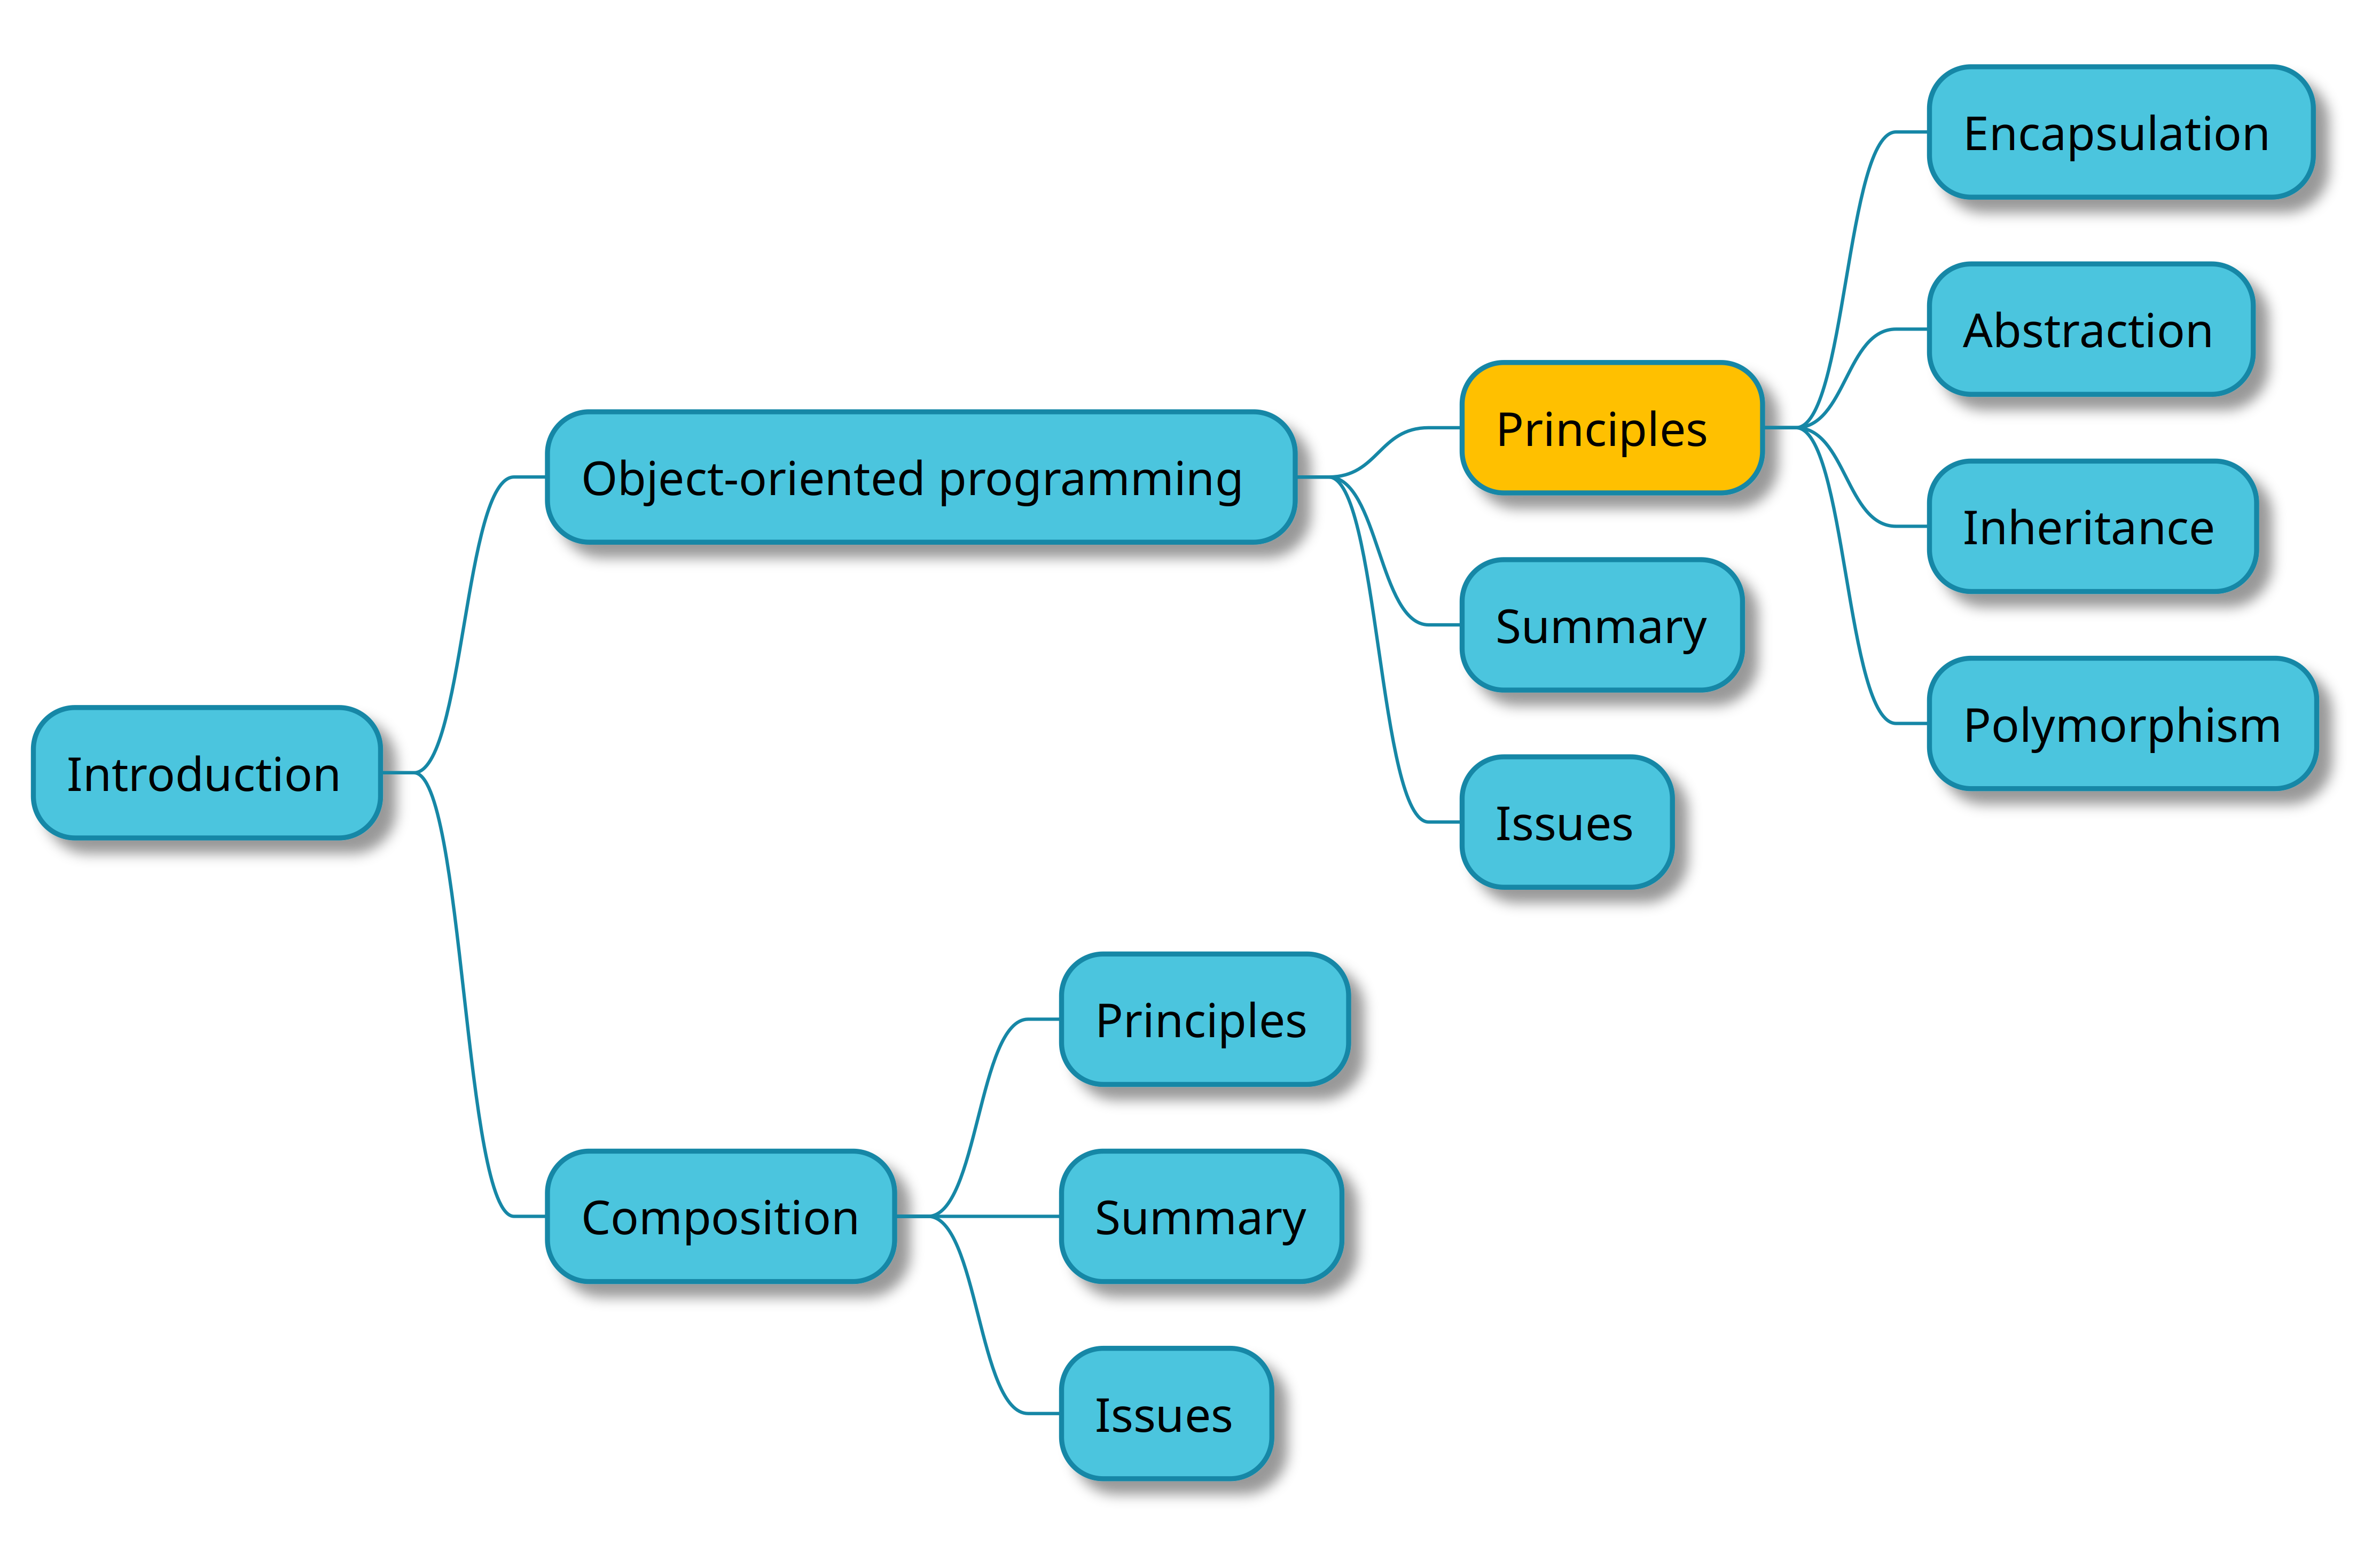
\includegraphics[width=\paperwidth]{src/session--composition-and-inheritance/resources/summary-oop-principles.png}}
\end{frame}

\begin{frame}
    \frametitle{Object-oriented programming}
    \framesubtitle{OOP Principles}

    \begin{itemize}[<+->]
        \item Encapsulation
        \item Abstraction
        \item Inheritance
        \item Polymorphism
    \end{itemize}
\end{frame}

\begin{frame}[fragile,c]
    \frametitle{Composition and inheritance}
    \framesubtitle{Map}

    \makebox[\linewidth]{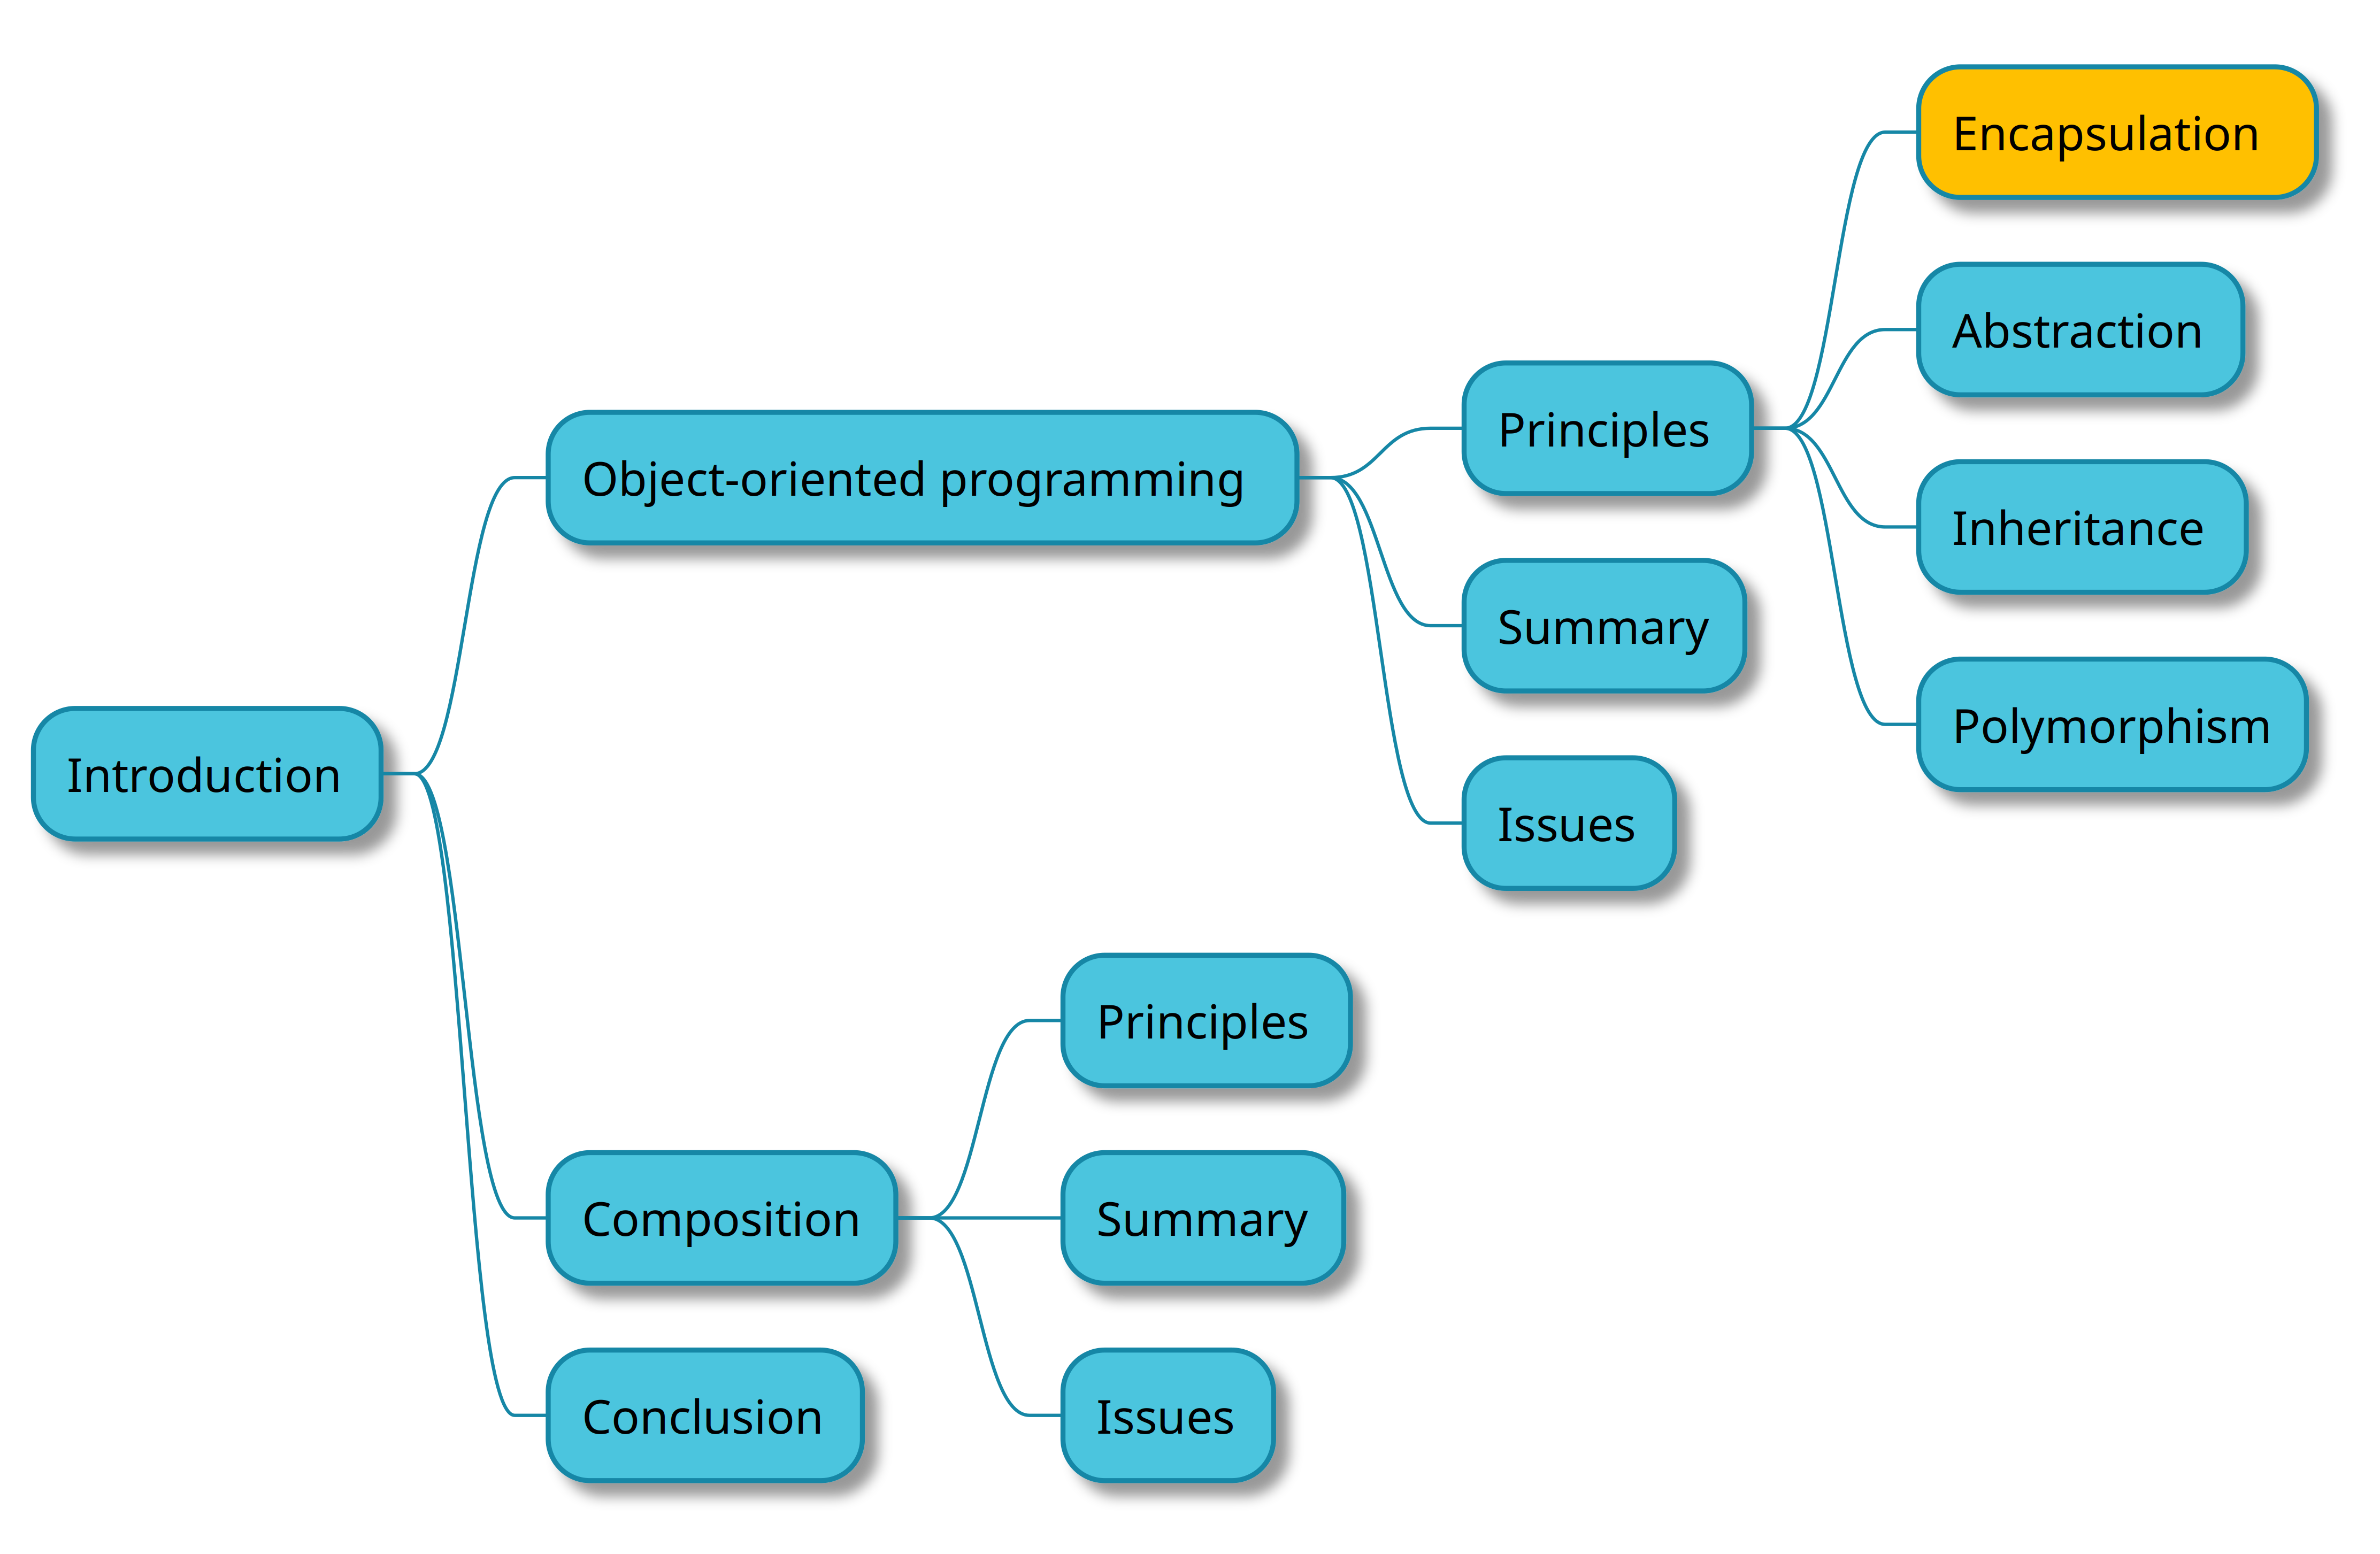
\includegraphics[width=\paperwidth]{src/session--composition-and-inheritance/resources/summary-oop-encapsulation.png}}
\end{frame}

\begin{frame}
    \frametitle{OOP Principles}
    \framesubtitle{Encapsulation}

    Encapsulation is an object-oriented programming concept that binds together the data and functions that manipulate the data,
    and that keeps both safe from outside interference and misuse.
\end{frame}

\begin{frame}
    \frametitle{OOP Principles}
    \framesubtitle{Encapsulation}

    \begin{itemize}
        \item Protect the internal state of an object access to the class variables\pause
              \textcolor{ecgrey!50}{
              \\Via the use of \texttt{getters} and \texttt{setters} methods}
        \pause
        \item Reduce software development complexity\pause
              \textcolor{ecgrey!50}{
              \\By hiding the implementation details and only exposing the operations, using a class becomes easy.}
        \pause
        \item The internal implementation of the class can be changed\pause
              \textcolor{ecgrey!50}{
              \\Without worrying about breaking the code that uses the class}
    \end{itemize}
\end{frame}

\begin{frame}[fragile,c]
    \frametitle{OOP Principles}
    \framesubtitle{Encapsulation / Getters \& setters}

    \begin{lstlisting}
    <?php

    class User
    {
        public function __construct(
            private string $name,
            private string $email,
        ) {}
    }
    \end{lstlisting}
\end{frame}

\begin{frame}[fragile,c]
    \frametitle{OOP Principles}
    \framesubtitle{Encapsulation / Getters \& setters}

    \begin{lstlisting}
    <?php

    class User
    {
        public function __construct(
            private string $name,
            private string $email,
        ) {}

        public function getName(): string
        {
            return $this->name;
        }

        public function setEmail(string $email): void
        {
            $this->email = $email;
        }
    }
    \end{lstlisting}
\end{frame}

\begin{frame}[fragile,c]
    \frametitle{Composition and inheritance}
    \framesubtitle{Map}

    \makebox[\linewidth]{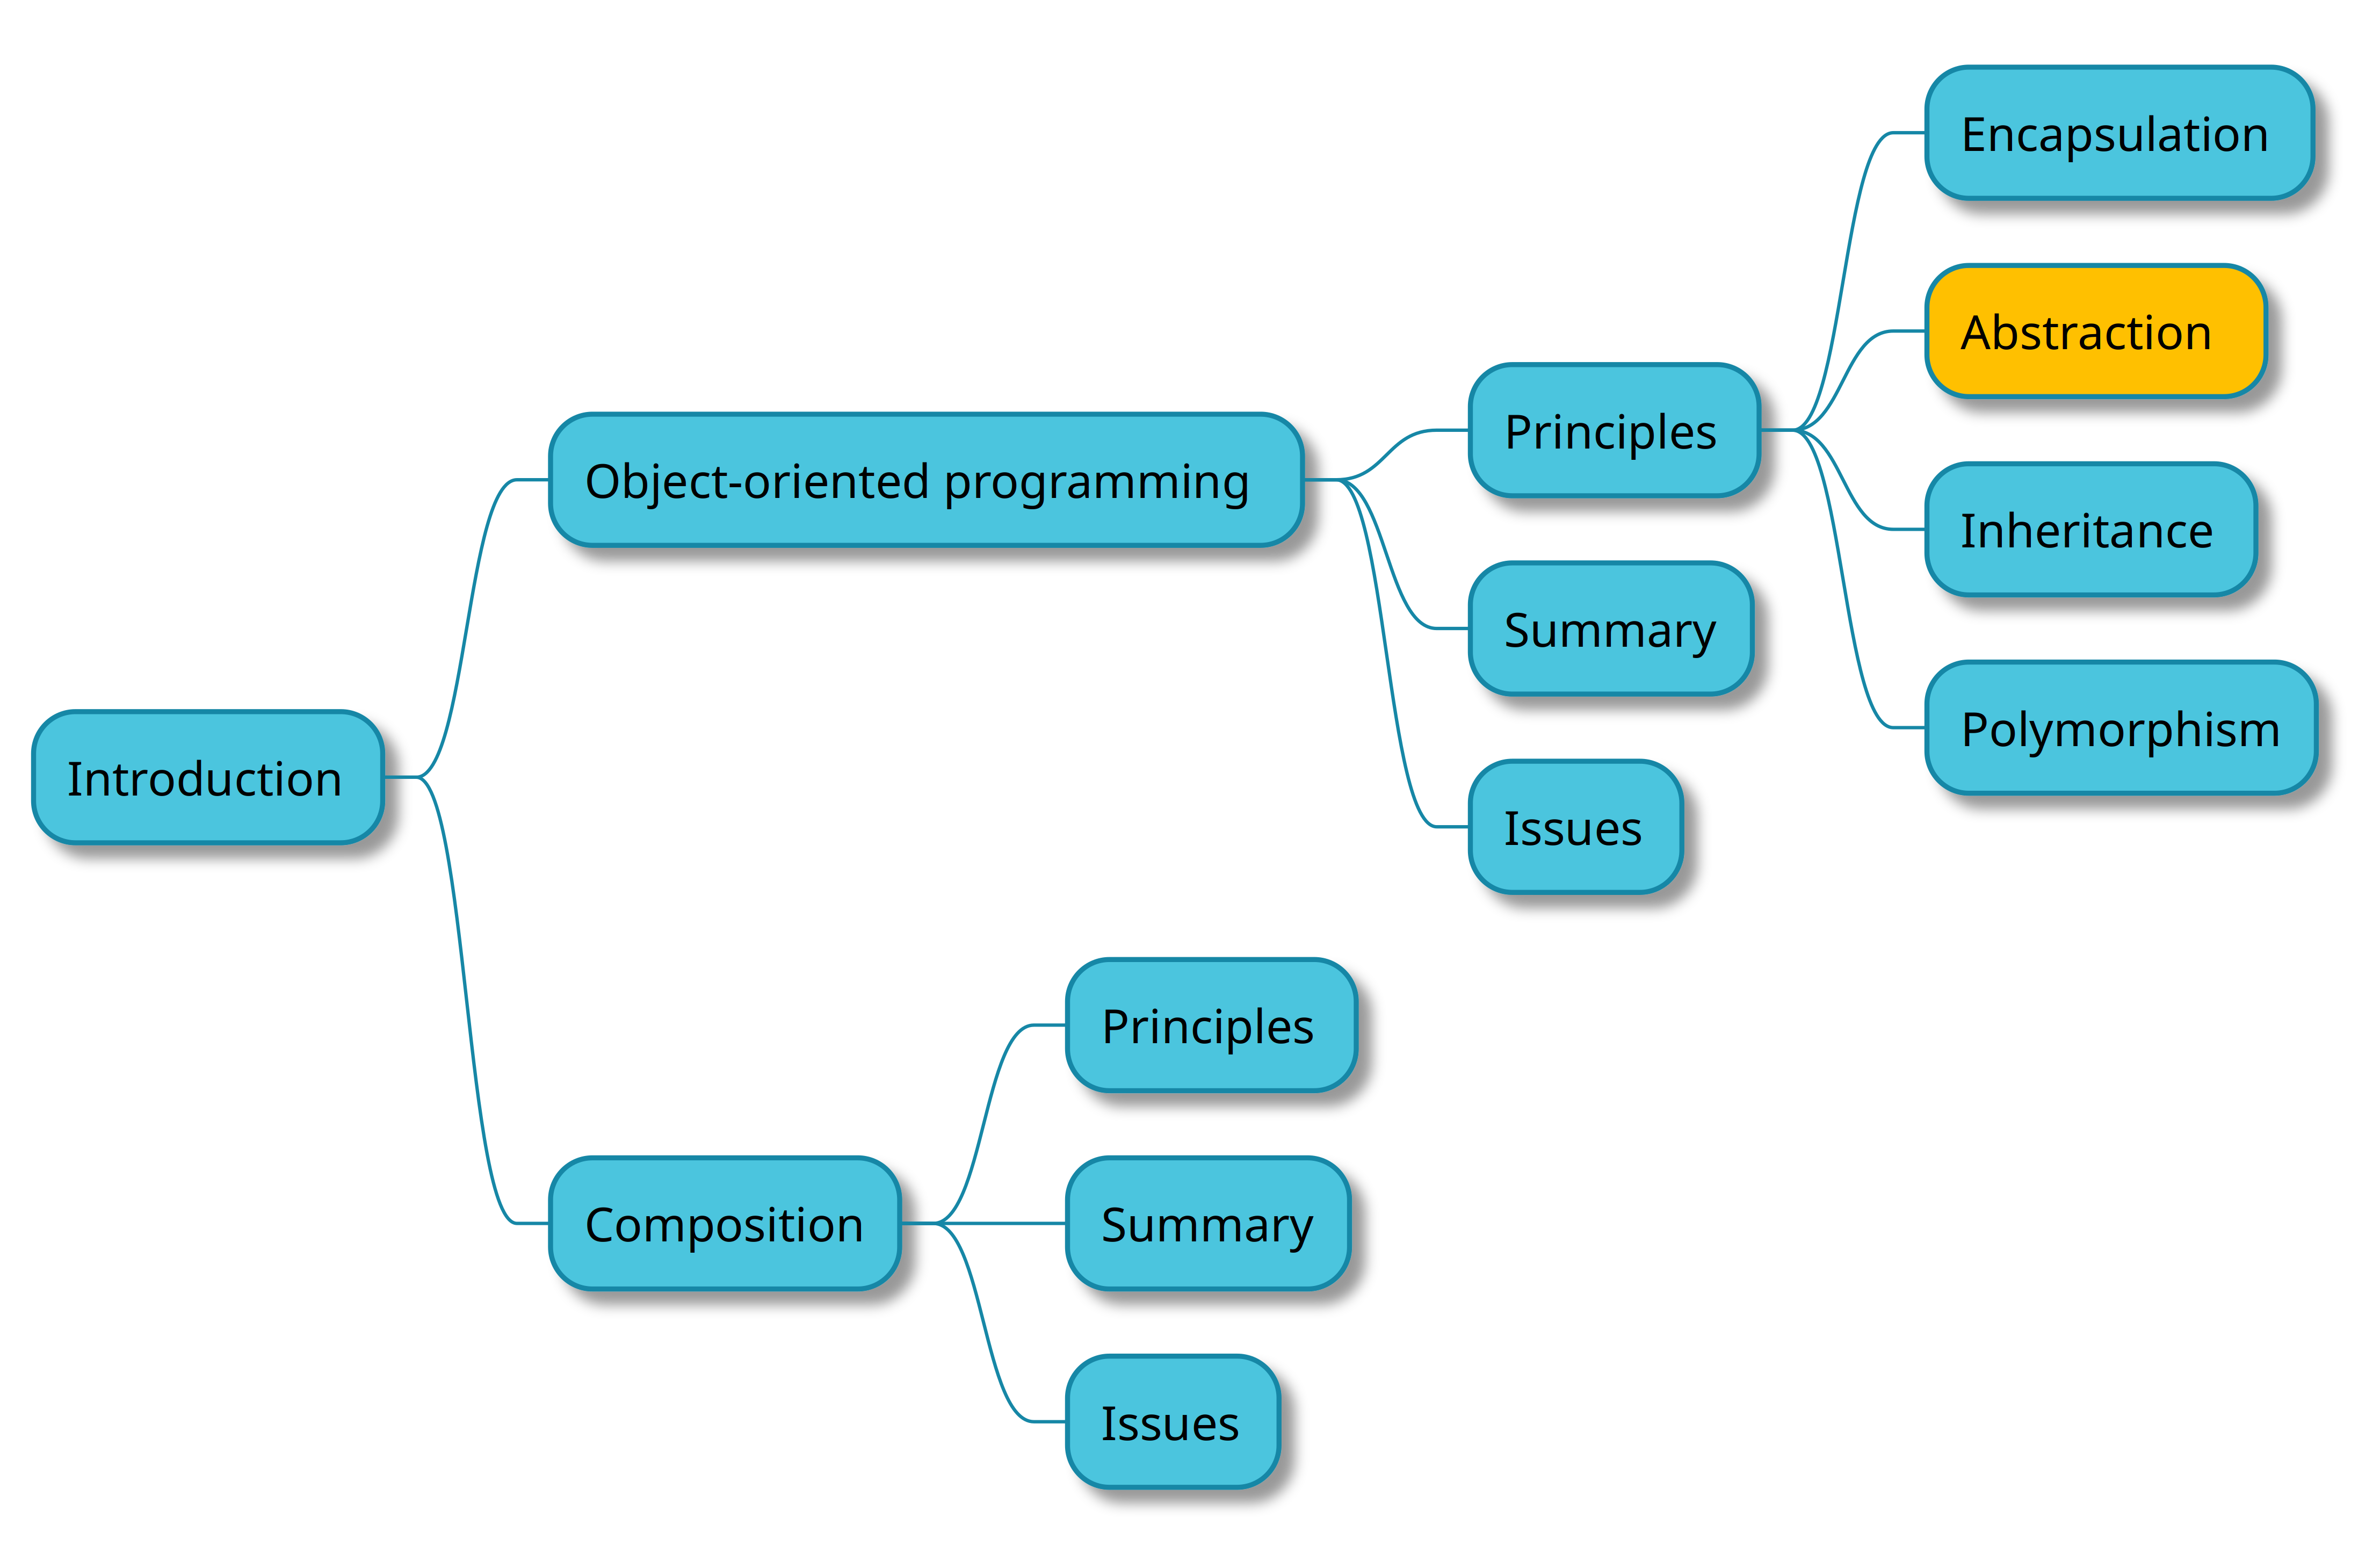
\includegraphics[width=\paperwidth]{src/session--composition-and-inheritance/resources/summary-oop-abstraction.png}}
\end{frame}

\begin{frame}
    \frametitle{OOP Principles}
    \framesubtitle{Abstraction}

    \begin{itemize}
        \item It’s easier to design a program when separating the interface from its implementation\pause
              \\\textcolor{ecgrey!50}{And focus on the interface only.}
        \pause
        \item This is like treating a system as a \textit{black box}\pause
              \\\textcolor{ecgrey!50}{Where it’s not important to understand the inner mechanisms in order to reap the benefits of using it.}
    \end{itemize}
\end{frame}

\begin{frame}
    \frametitle{OOP Principles}
    \framesubtitle{Abstraction}

    \begin{itemize}
        \item This process is called \textit{abstraction}\pause
              \\\textcolor{ecgrey!50}{Because we are abstracting away the implementation detail and only presenting a clean and \textit{easy-to-use} interface via the class methods.}
        \pause
        \item \textit{Abstraction} helps isolate the impact of changes made to the code\pause
              \\\textcolor{ecgrey!50}{So that if something goes wrong, the change will only affect the implementation details and not the outside code.}
    \end{itemize}
\end{frame}

\begin{frame}[fragile,c]
    \frametitle{OOP Principles}
    \framesubtitle{Abstraction / Using interfaces}

    \begin{lstlisting}
    <?php

    $user = new User('patrick', 'user@example.com');

    function printPrettyUsername(User $user): string
    {
        return ucfirst($user->getName());
    }

    printUsername($user); // Patrick
    \end{lstlisting}
\end{frame}

\begin{frame}[fragile,c]
    \frametitle{OOP Principles}
    \framesubtitle{Abstraction / Using interfaces}

    \begin{lstlisting}
    <?php

    interface UserInterface {
        public function getName(): string;
        public function setEmail(string $email): void;
    }

    class User implements UserInterface
    {
        /* Same content as before */
    }

    $user = new User('patrick', 'user@example.com');

    function printPrettyUsername(UserInterface $user): string
    {
        return ucfirst($user->getName());
    }

    printUsername($user); // Patrick
    \end{lstlisting}
\end{frame}

\begin{frame}[fragile,c]
    \frametitle{Composition and inheritance}
    \framesubtitle{Map}

    \makebox[\linewidth]{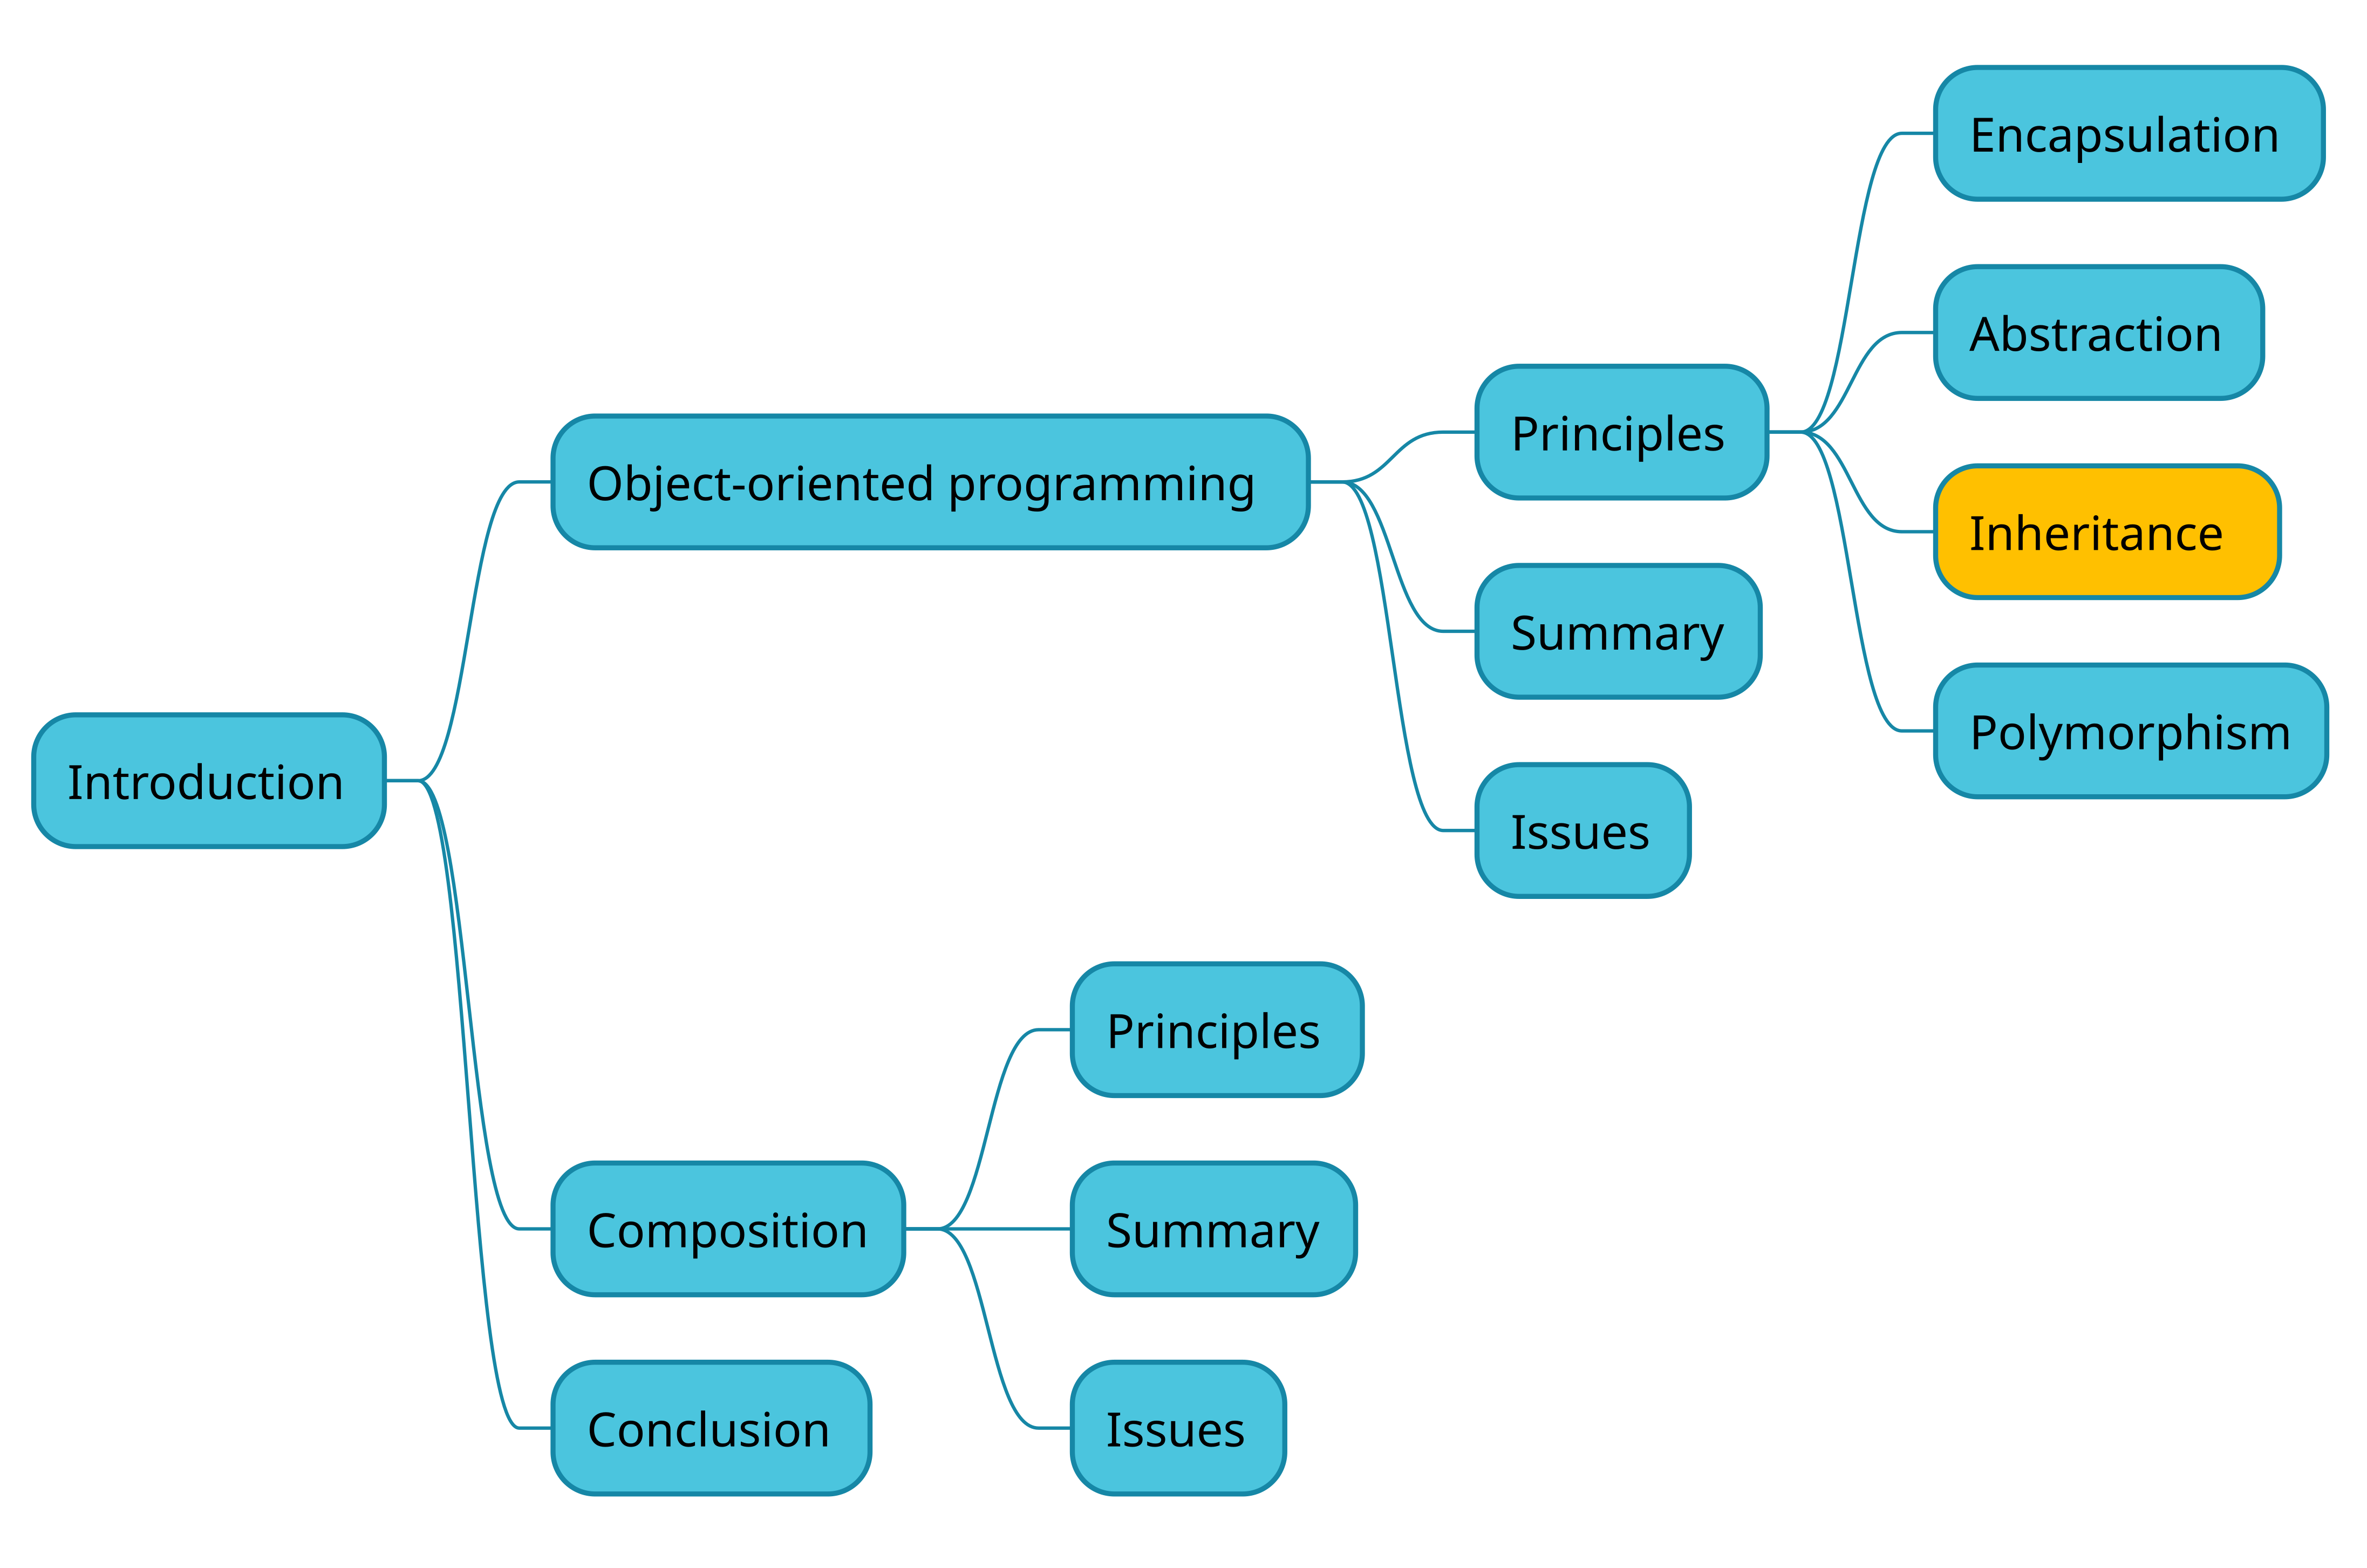
\includegraphics[width=\paperwidth]{src/session--composition-and-inheritance/resources/summary-oop-inheritance.png}}
\end{frame}

\begin{frame}
    \frametitle{OOP Principles}
    \framesubtitle{Inheritance}

    \begin{itemize}
        \item It is fundamental to OOP\pause
              \\\textcolor{ecgrey!50}{A programming language may have objects and messages, but without inheritance it's not object-oriented (\textit{merely “object-based”, but still polymorphic}).}
        \pause
        \item Inheritance serves two purposes: semantics and mechanics.
        \pause
        \item Inheritance will affect the way many classes and objects relate to each other.
        \pause
        \item Inheritance is achieved by \textit{extending} another class
    \end{itemize}
\end{frame}

\begin{frame}
    \frametitle{OOP Principles}
    \framesubtitle{Inheritance}

    \begin{itemize}[<+->]
        \item When \textit{extending} a class, the subclass inherits methods, properties and constants from the parent class.
        \item Permits the implementation of additional functionality in similar objects without the need to reimplement all of the shared functionality. (\textit{DRY})
        \item The visibility of methods, properties and constants can be relaxed.
    \end{itemize}
\end{frame}

\begin{frame}[fragile,c]
    \frametitle{OOP Principles}
    \framesubtitle{Inheritance / Example}

    \begin{lstlisting}
<?php

class OfficialUser extends User
{
    public function getName(): string
    {
        return sprintf('Mr %s', parent::getName());
    }

    public function getBadgeId(): int
    {
        return array_reduce(
            str_split($this->getName()),
            static fn (int $s, string $letter): int => $s + ord($letter),
            0
        );
    }
}

$user = new OfficialUser('patrick', 'user@example.com');

echo $user->getName(); // Mr patrick
echo $user->getBadgeId(); // 973
    \end{lstlisting}
\end{frame}

\begin{frame}[fragile,c]
    \frametitle{OOP Principles}
    \framesubtitle{Inheritance / UML representation}

    \begin{center}
        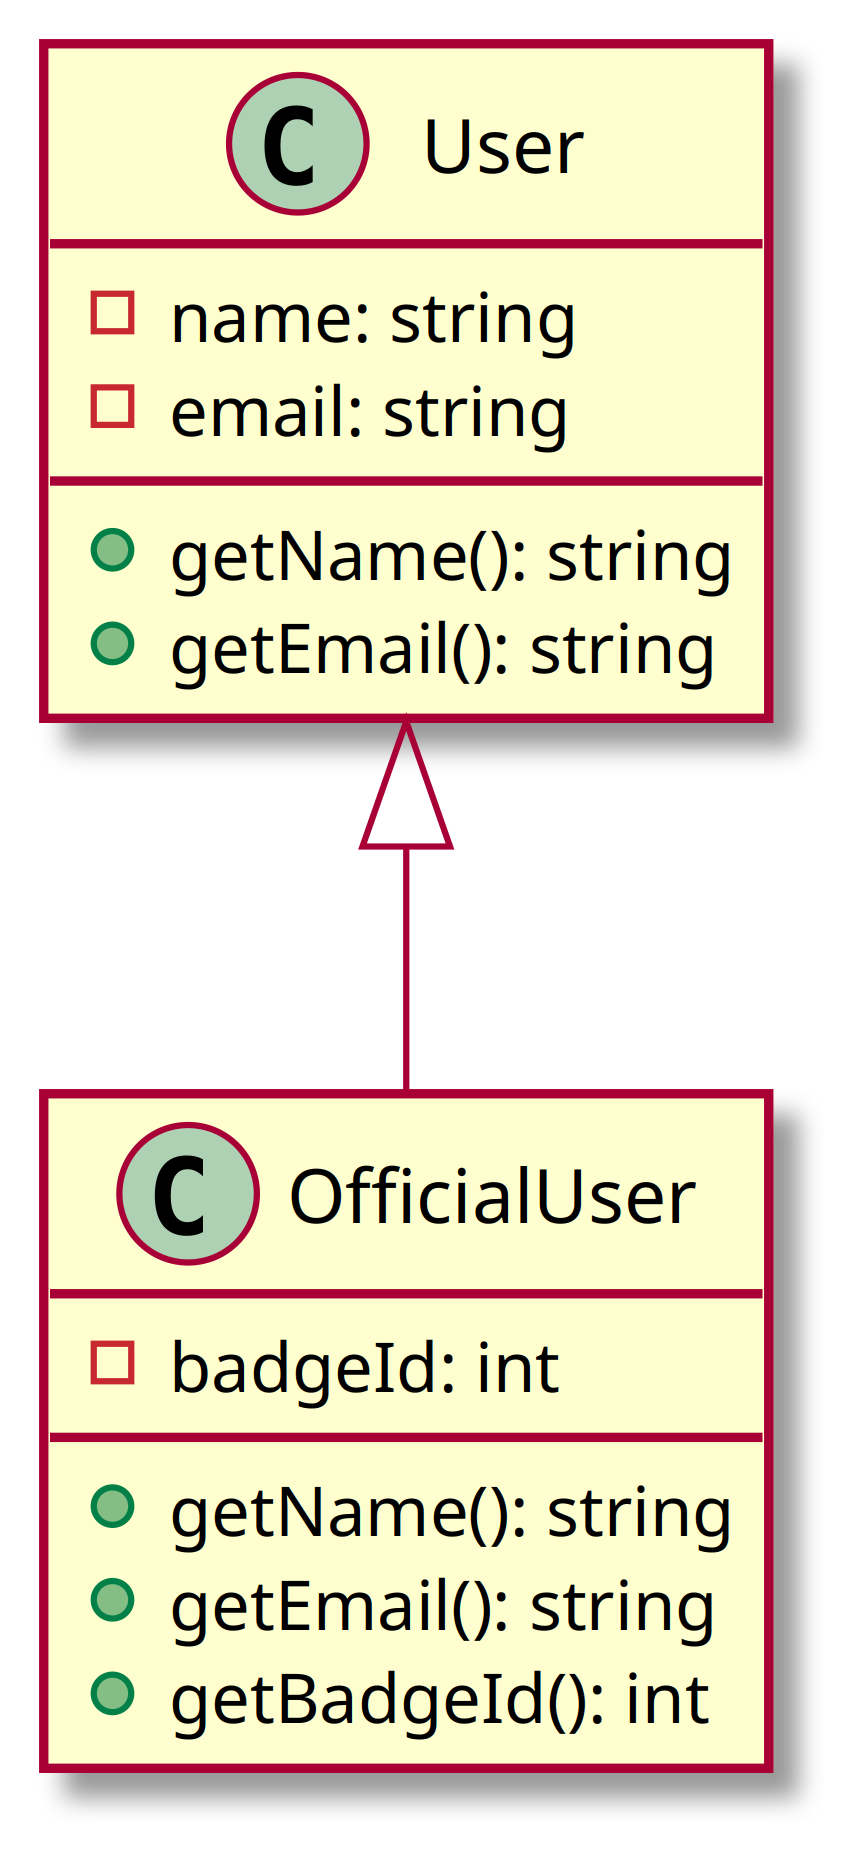
\includegraphics[height=.75\textheight]{src/session--composition-and-inheritance/resources/Inheritance.png}
    \end{center}
\end{frame}

\begin{frame}[fragile,c]
    \frametitle{Composition and inheritance}
    \framesubtitle{Map}

    \makebox[\linewidth]{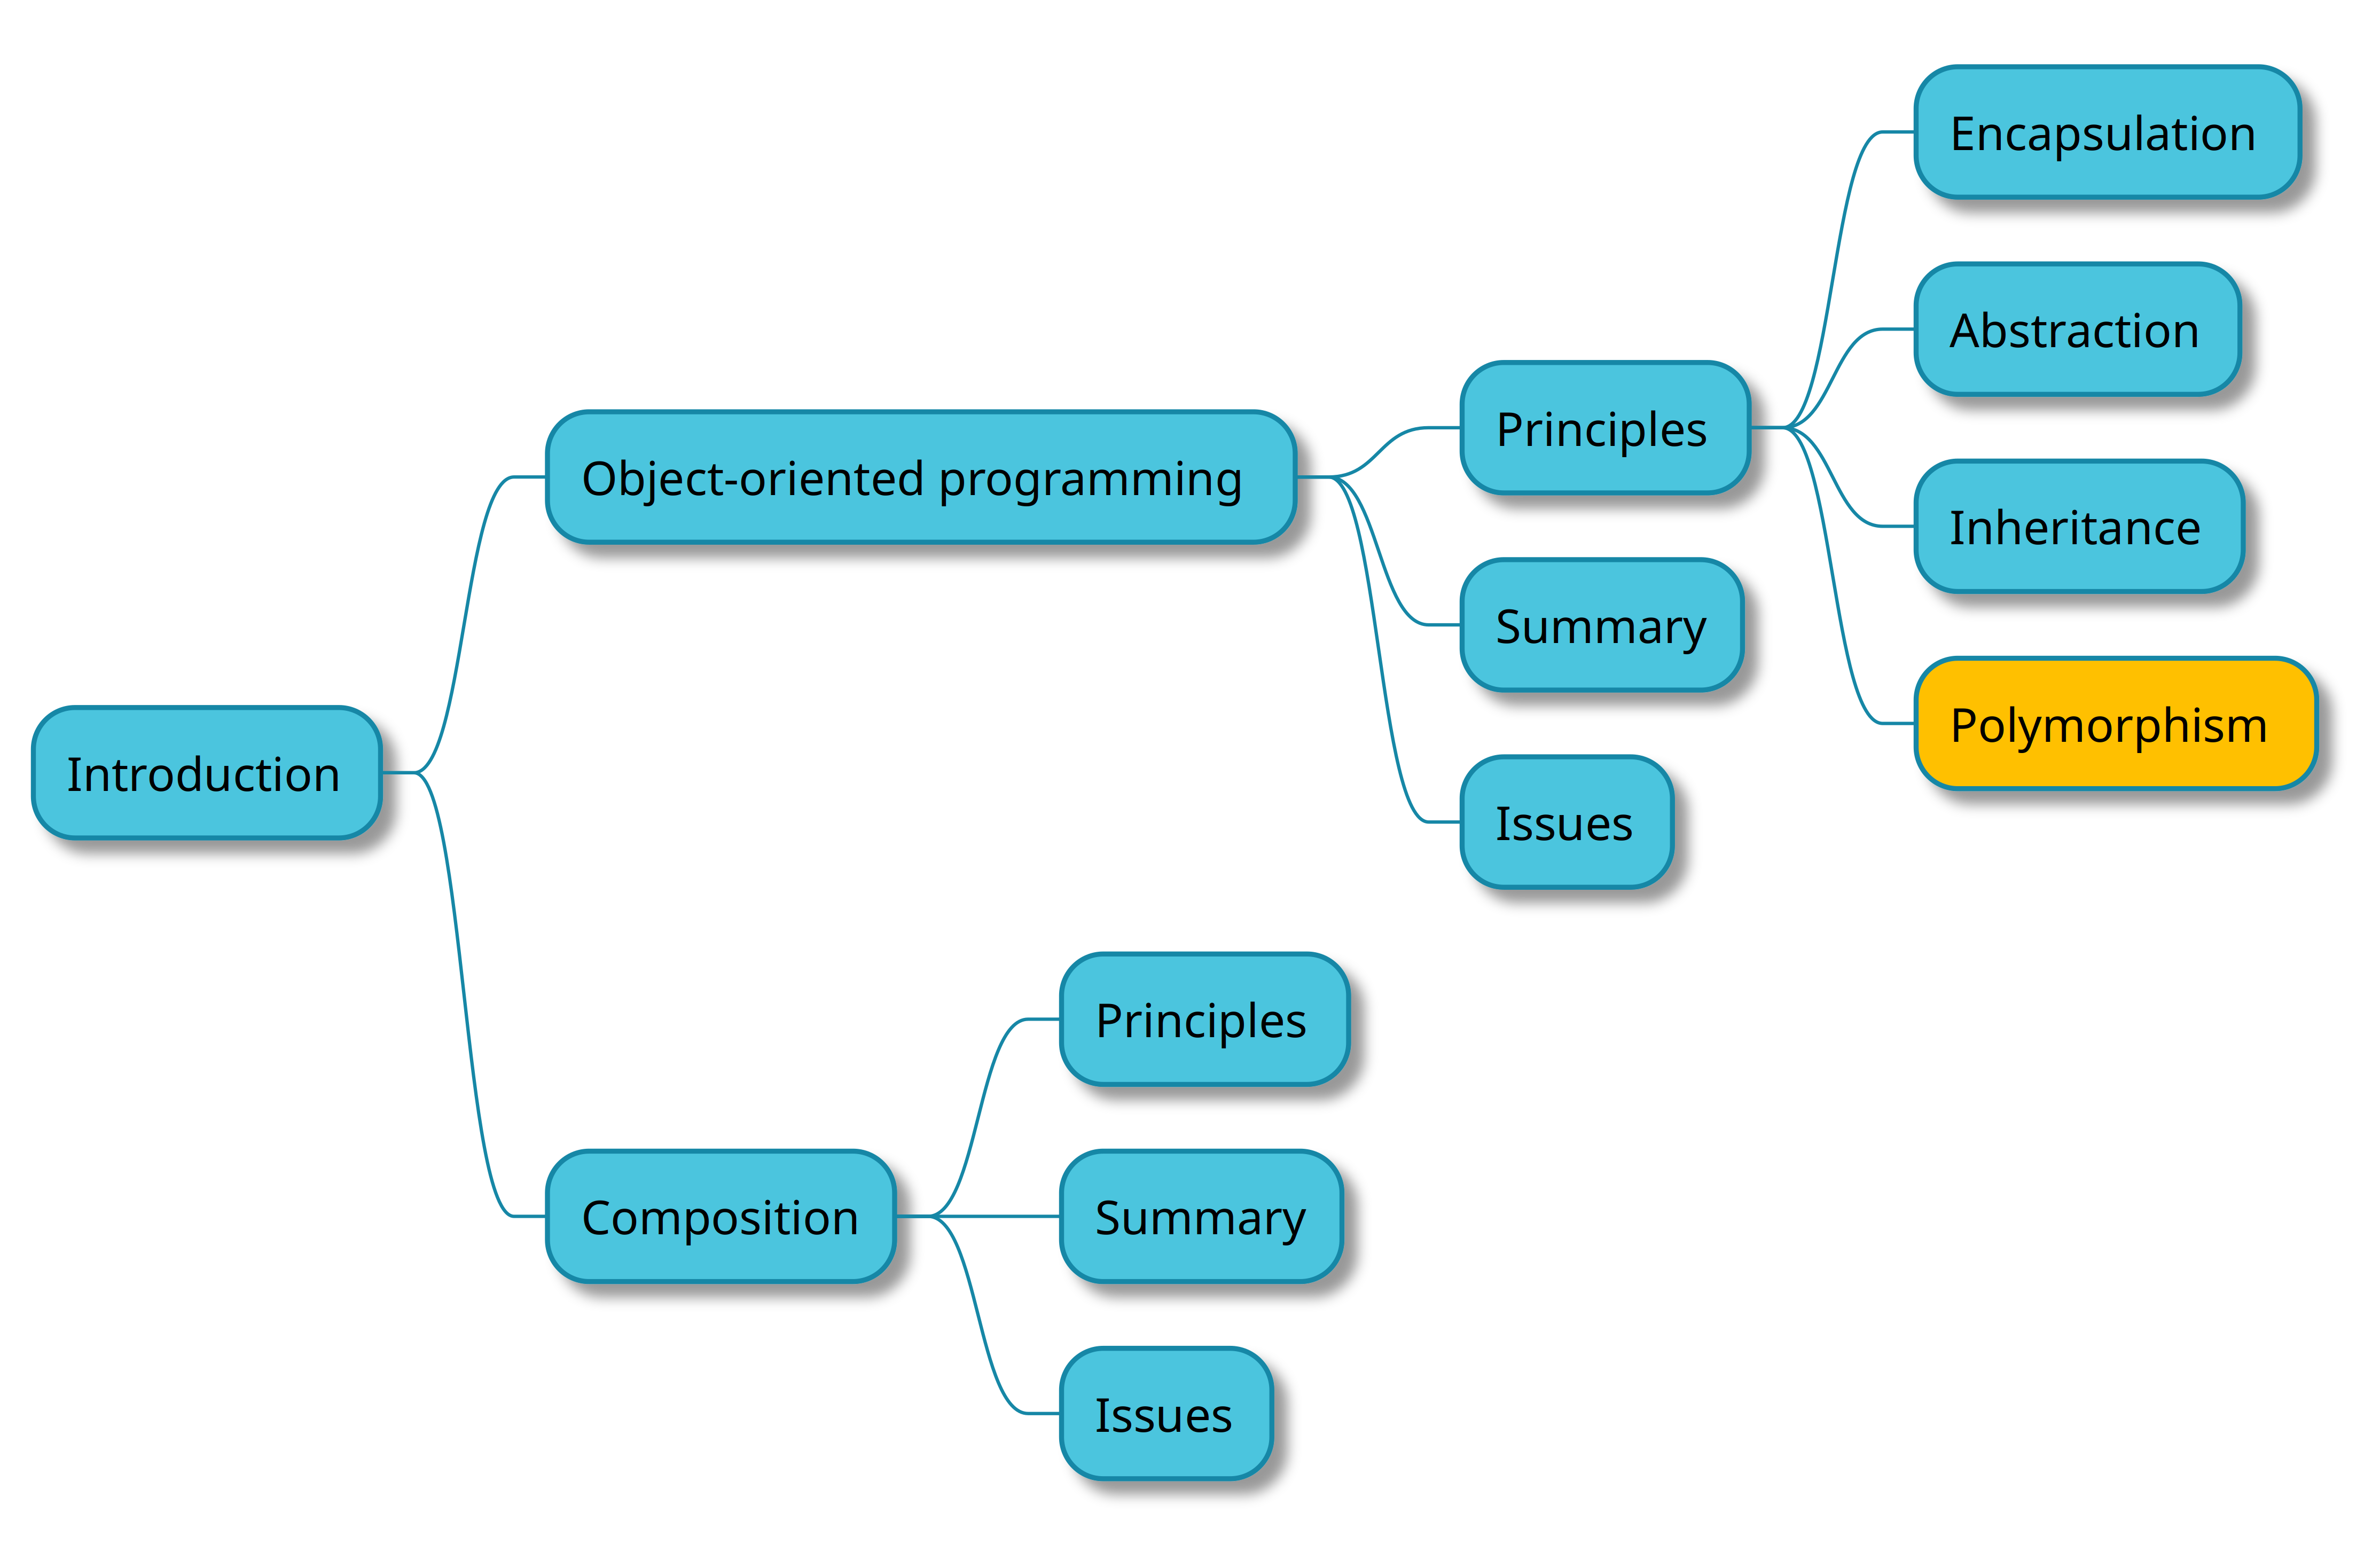
\includegraphics[width=\paperwidth]{src/session--composition-and-inheritance/resources/summary-oop-polymorphism.png}}
\end{frame}

\begin{frame}
    \frametitle{OOP Principles}
    \framesubtitle{Polymorphism}

    \begin{itemize}[<+->]
        \item Polymorphism is a Greek word that literally means "many forms".
        \item Polymorphism is closely related to inheritance.
        \item Polymorphism allows objects of different classes to respond differently based on the same message.
        \item To implement polymorphism in PHP, you can use either \texttt{abstract} classes or \texttt{interfaces}.
    \end{itemize}
\end{frame}

\begin{frame}[fragile,c]
    \frametitle{OOP Principles}
    \framesubtitle{Polymorphism / With an abstract class}

    \begin{lstlisting}
<?php

abstract class Person {
    abstract public function greet(): string;
}

class Dutch extends Person
{
    public function greet(): string { return 'Hallo!'; }
}

class English extends Person
{
    public function greet(): string { return 'Hello!'; }
}

$dutch = new Dutch;
$english = new English;

var_dump($dutch instanceof Person); // true
var_dump($english instanceof Person); // true
    \end{lstlisting}
\end{frame}

\begin{frame}[fragile,c]
    \frametitle{OOP Principles}
    \framesubtitle{Polymorphism / With an abstract class}

    \begin{lstlisting}
<?php

abstract class Person {
    abstract public function greet(): string;
}

class Dutch extends Person
{
    public function greet(): string { return 'Hallo!'; }
}

class English extends Person
{
    public function greet(): string { return 'Hello!'; }
}

$greetings = array_map(
    static fn (Person $person): string => $person->greet(),
    [new Dutch, new English]
); // ['Hallo!', 'Hello!']
    \end{lstlisting}
\end{frame}

\begin{frame}[fragile,c]
    \frametitle{OOP Principles}
    \framesubtitle{Polymorphism / With an interface}

    \begin{lstlisting}
<?php

interface Greatable
{
    public function greet(): string;
}

class Dutch implements Greatable
{
    public function greet(): string { return 'Hallo!'; }
}

class English implements Greatable
{
    public function greet(): string { return 'Hello!'; }
}

$dutch = new Dutch;
$english = new English;

var_dump($dutch instanceof Greatable); // true
var_dump($english instanceof Greatable); // true
    \end{lstlisting}
\end{frame}

\begin{frame}[fragile,c]
    \frametitle{OOP Principles}
    \framesubtitle{Polymorphism / With an interface}

    \begin{lstlisting}
<?php

interface Greatable
{
    public function greet(): string;
}

class Dutch implements Greatable
{
    public function greet(): string { return 'Hallo!'; }
}

class English implements Greatable
{
    public function greet(): string { return 'Hello!'; }
}

$greetings = array_map(
    static fn (Greatable $user): string => $user->greet(),
    [new Dutch, new English]
); // ['Hallo!', 'Hello!']
    \end{lstlisting}
\end{frame}

\begin{frame}[fragile,c]
    \frametitle{Composition and inheritance}
    \framesubtitle{Map}

    \makebox[\linewidth]{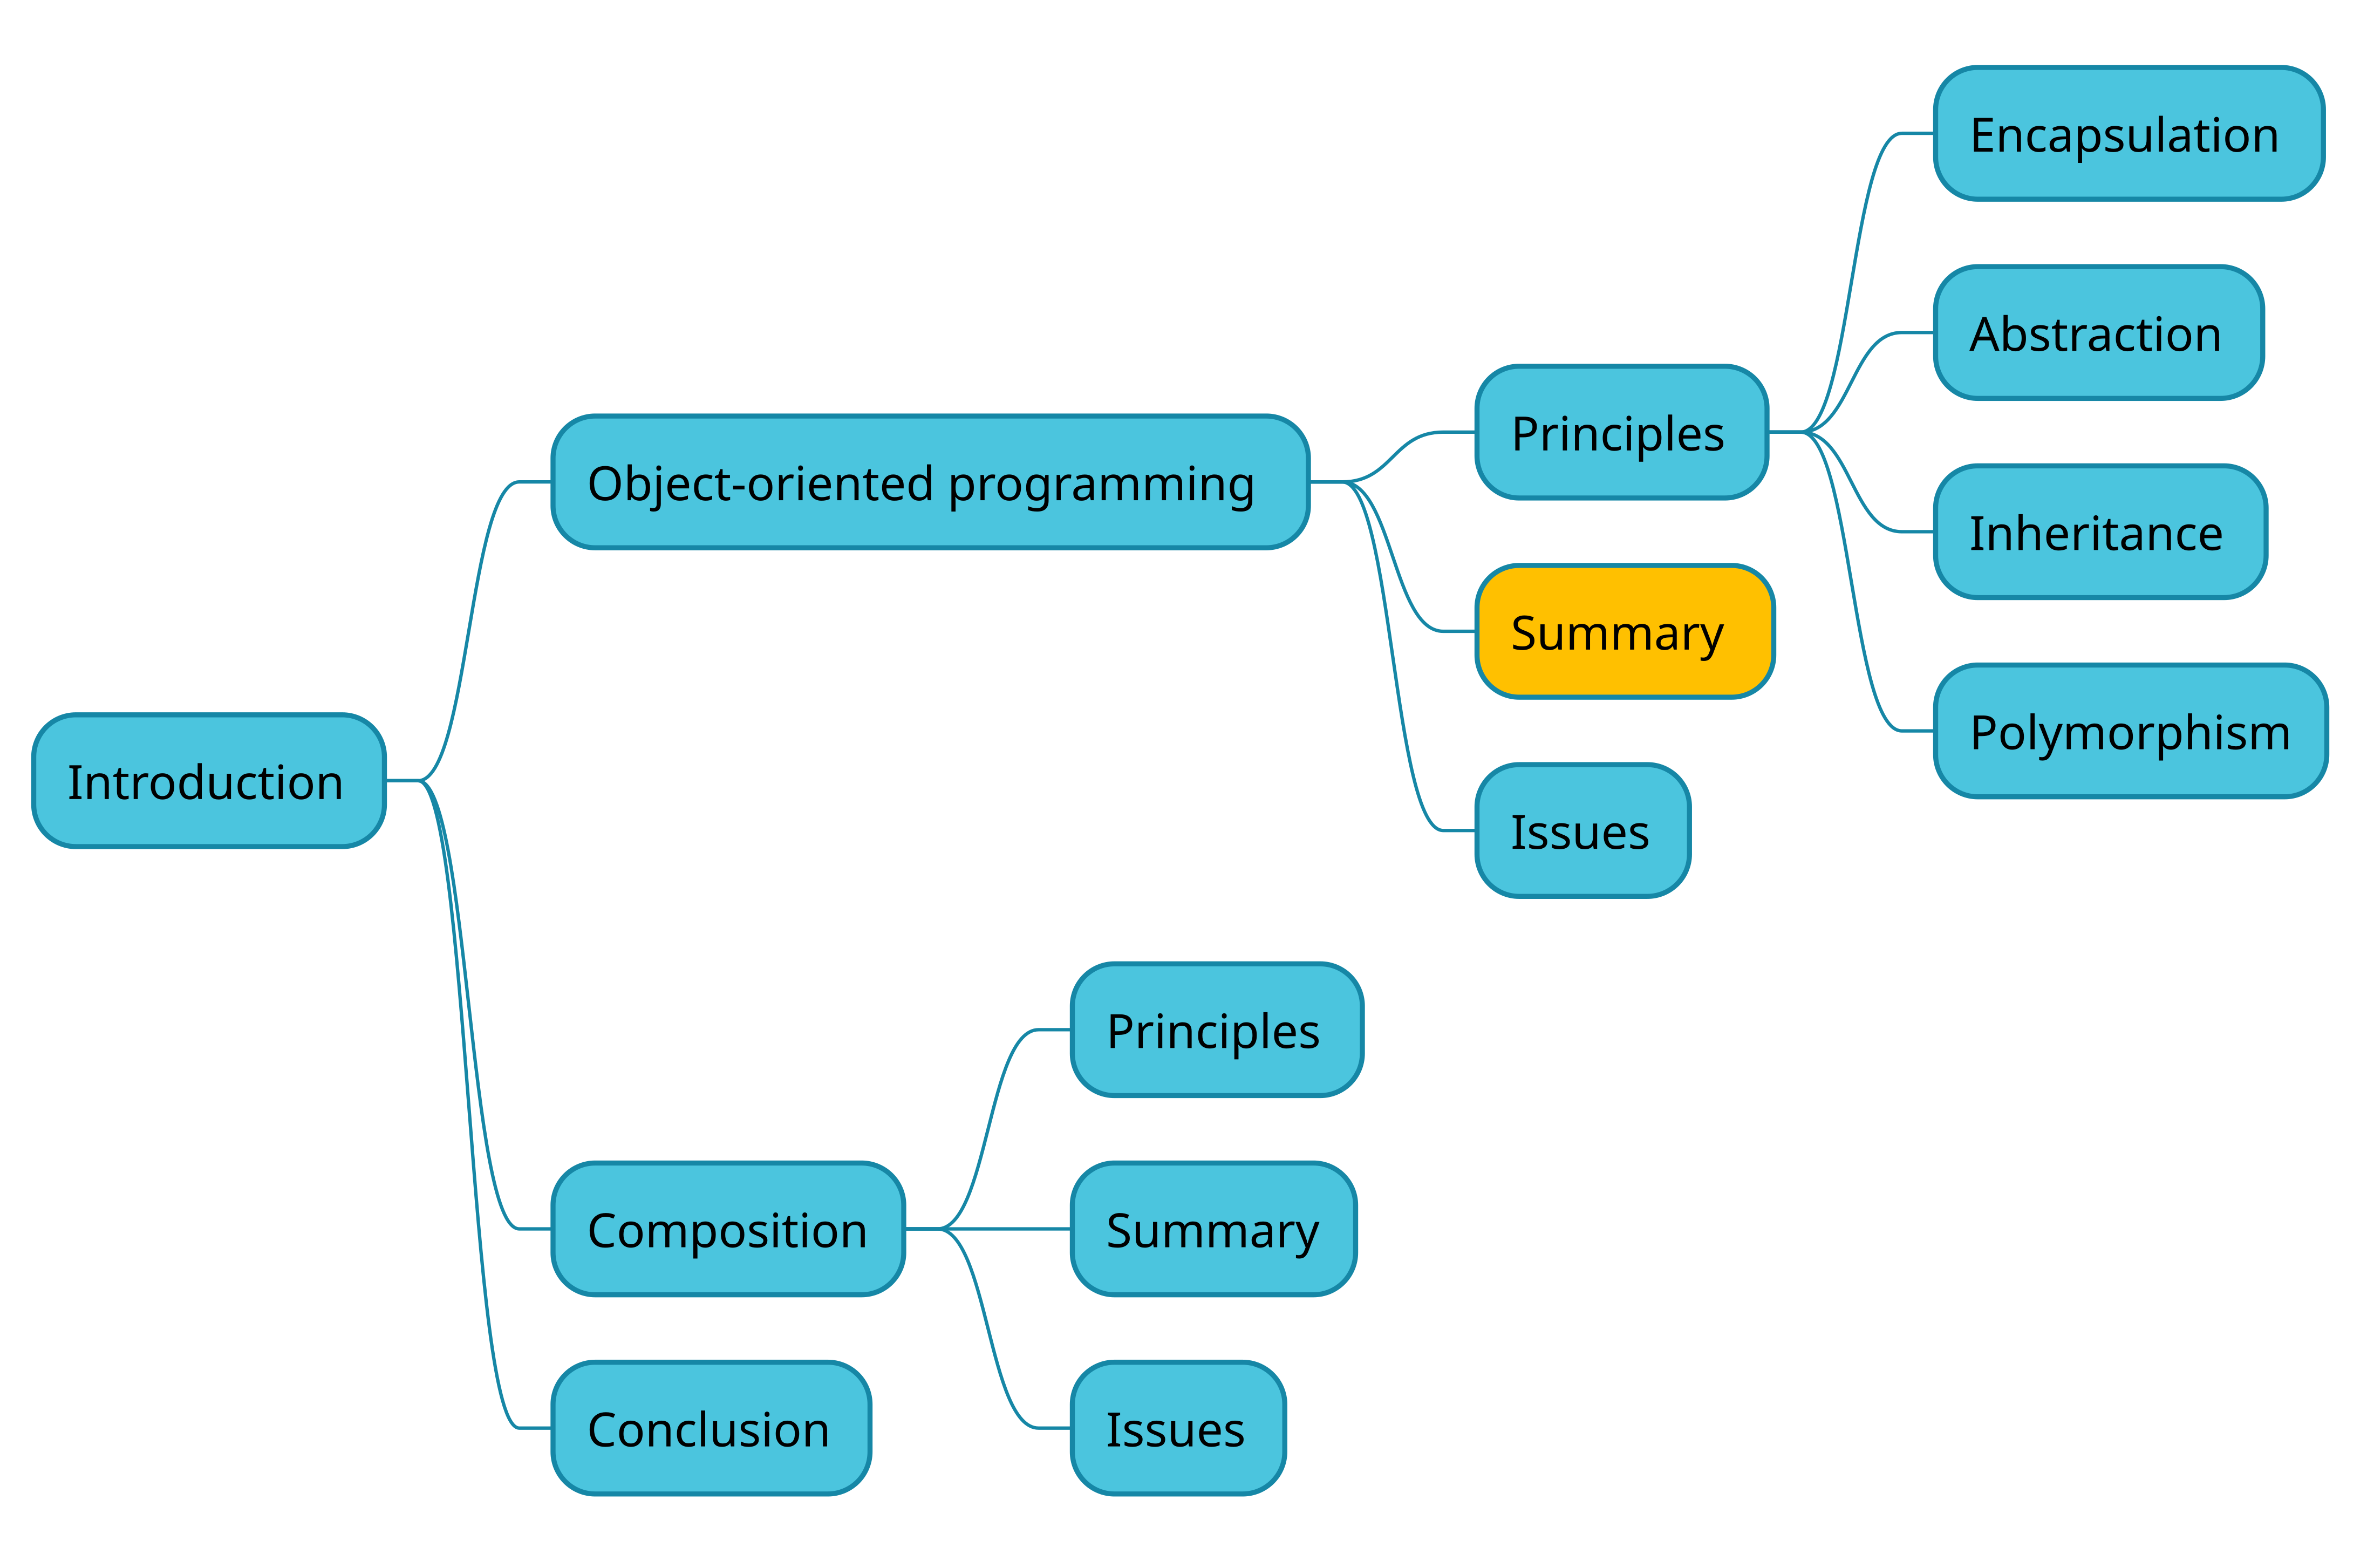
\includegraphics[width=\paperwidth]{src/session--composition-and-inheritance/resources/summary-oop-summary.png}}
\end{frame}

\begin{frame}
    \frametitle{OOP Principles}
    \framesubtitle{At a glance}

    \begin{itemize}
        \item Encapsulation\pause: \texttt{public}, \texttt{protected}, \texttt{private}
        \pause
        \item Abstraction\pause: \texttt{interface}
        \pause
        \item Inheritance\pause: \texttt{extends}
        \pause
        \item Polymorphism\pause: \texttt{abstract}
    \end{itemize}
\end{frame}

\begin{frame}[c]
    \begin{center}
        \Huge One day, I’m going to live in \textit{theory} \pause because in \textit{theory} everything goes perfectly.
    \end{center}
\end{frame}

\begin{frame}[fragile,c]
    \frametitle{Composition and inheritance}
    \framesubtitle{Map}

    \makebox[\linewidth]{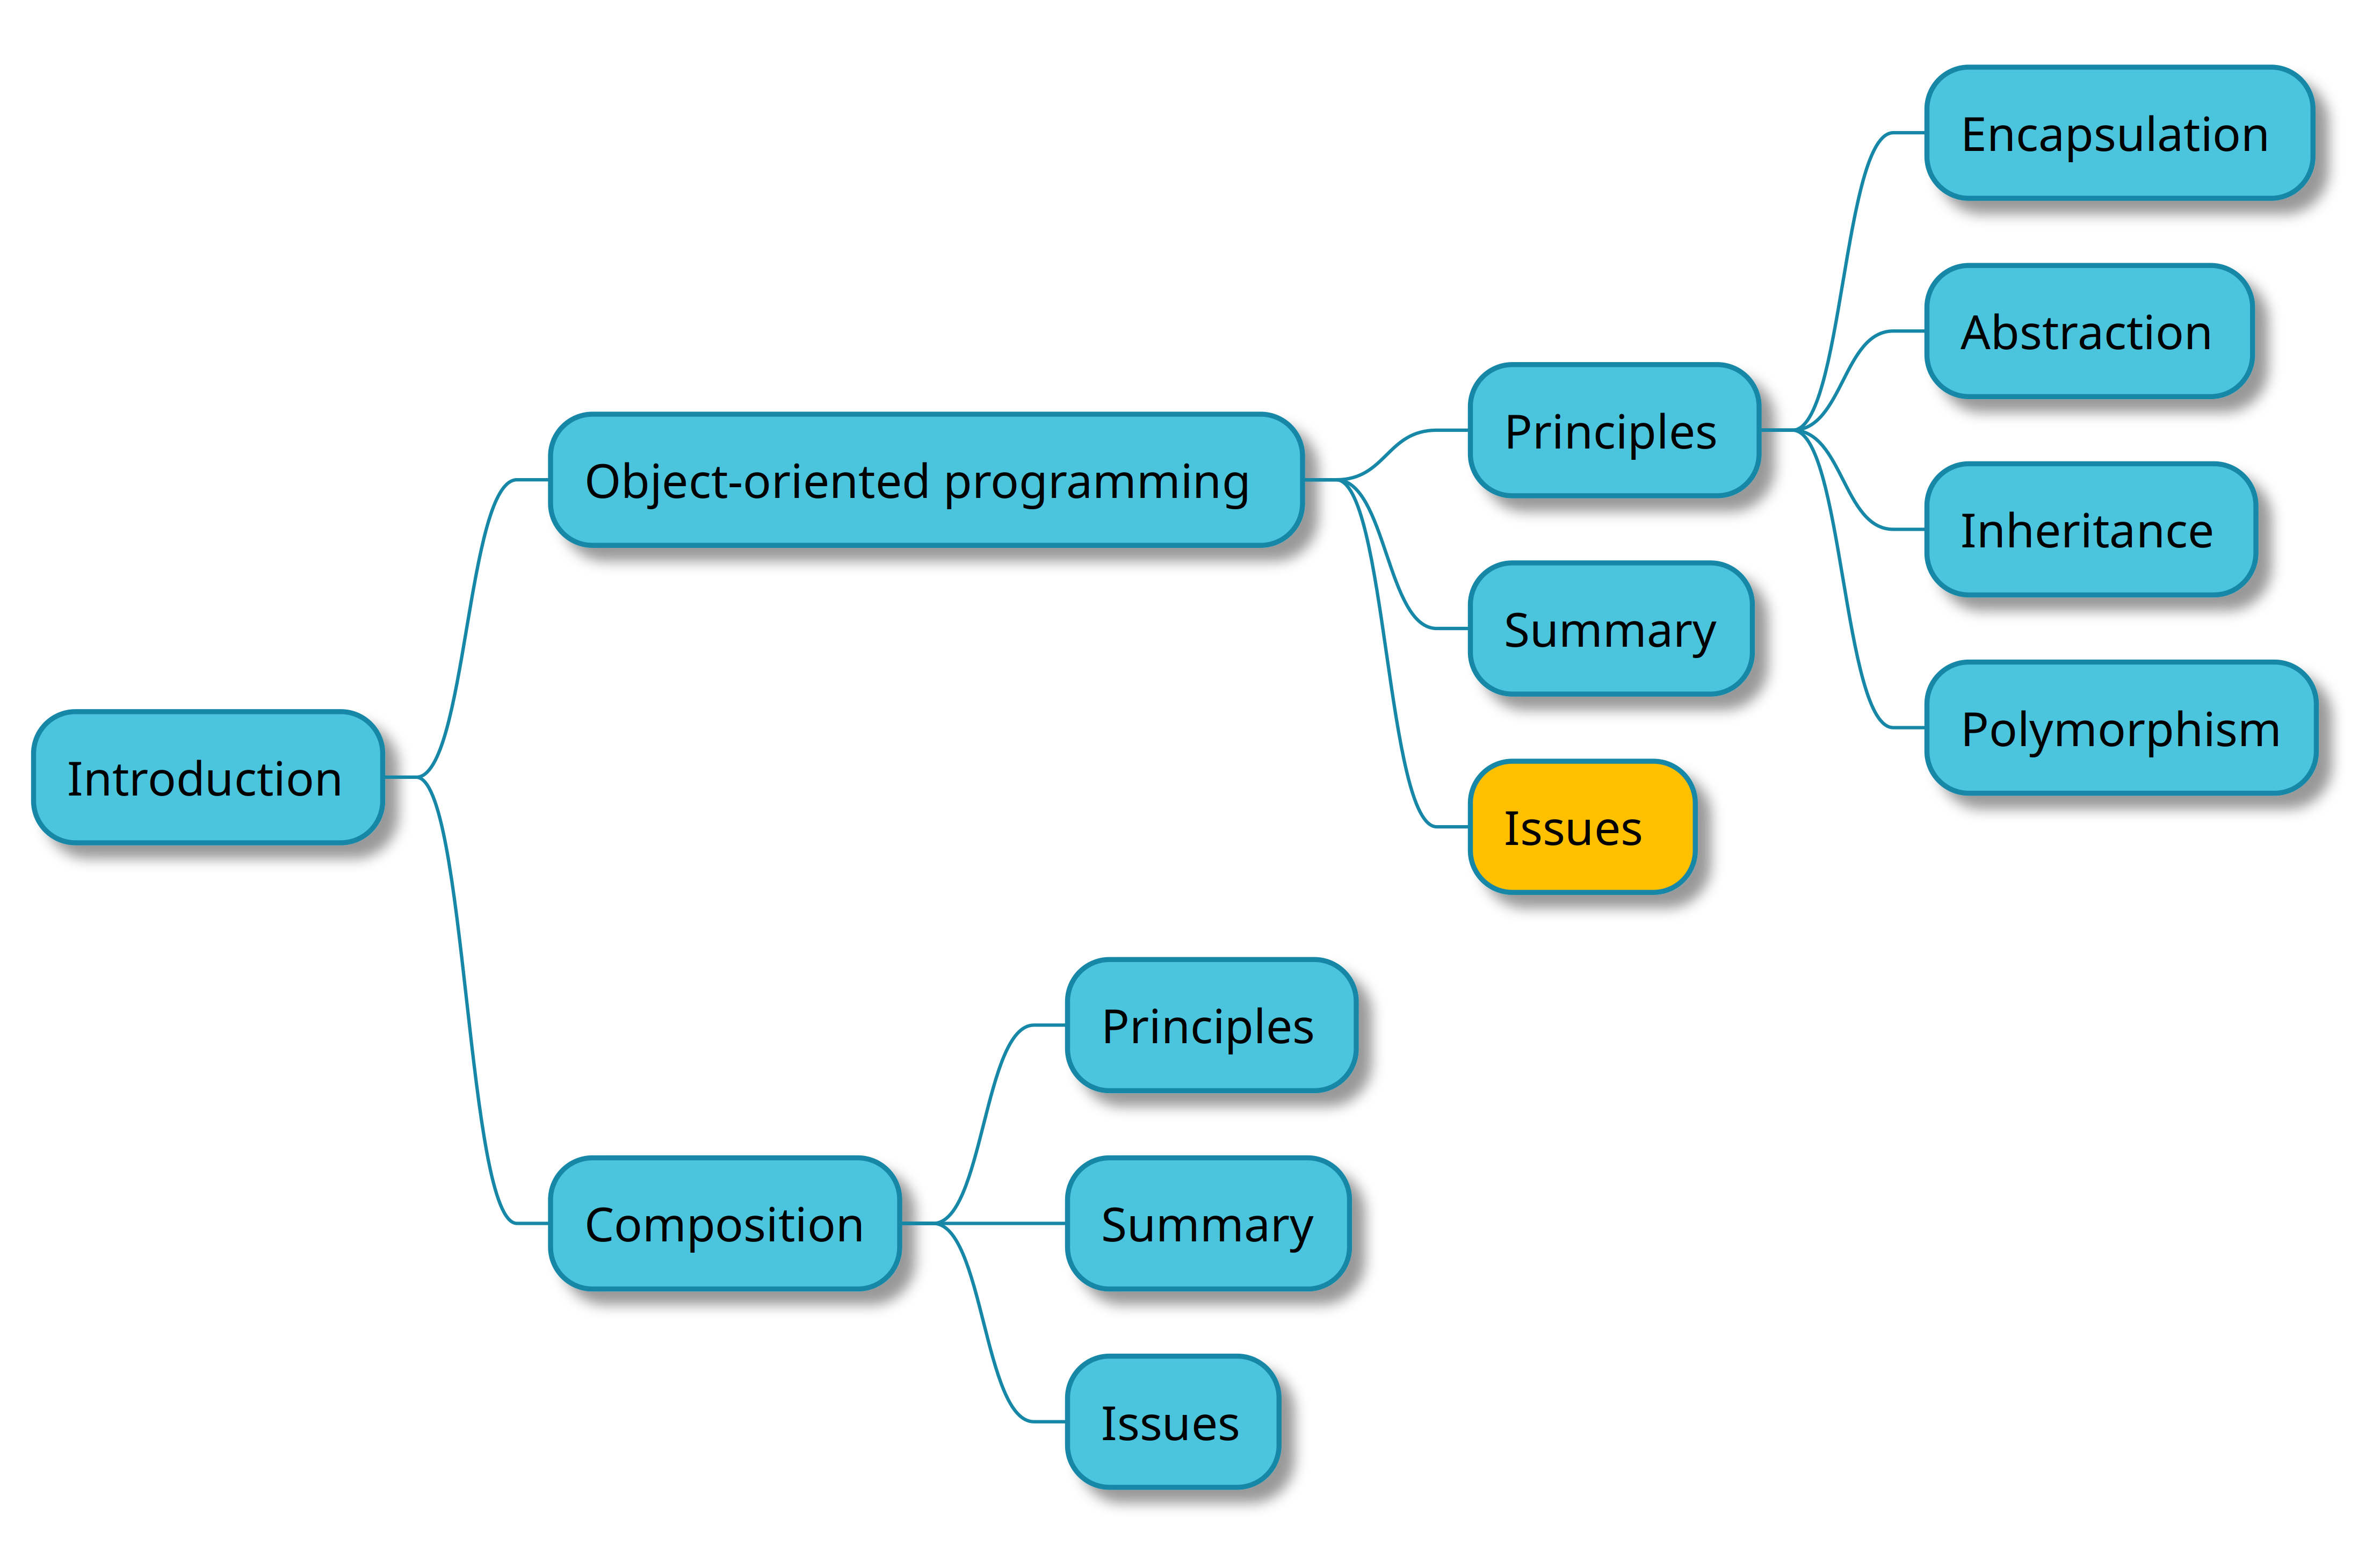
\includegraphics[width=\paperwidth]{src/session--composition-and-inheritance/resources/summary-oop-issues.png}}
\end{frame}

\begin{frame}
    \frametitle{OOP}
    \framesubtitle{Issues}

    \begin{itemize}[<+->]
        \item The \textit{Yo-Yo} problem
        \item It breaks encapsulation
        \item The inheritance of unnecessary methods
        \item Lack of flexibility
        \item Creates an \texttt{Is-a} relation
    \end{itemize}
\end{frame}

\begin{frame}
    \frametitle{OOP}
    \framesubtitle{Issues / The \textit{Yo-Yo} problem}

    Anti-pattern that occurs when a programmer has to read and understand
    a program whose inheritance graph is so long and complicated that the
    programmer has to keep flipping between many different class definitions
    in order to follow the control flow of the program.
\end{frame}

\begin{frame}[fragile,c]
    \frametitle{OOP}
    \framesubtitle{Issues / The \textit{Yo-Yo} problem}

    \noindent
    \begin{minipage}{.20\textwidth}
        \begin{center}
            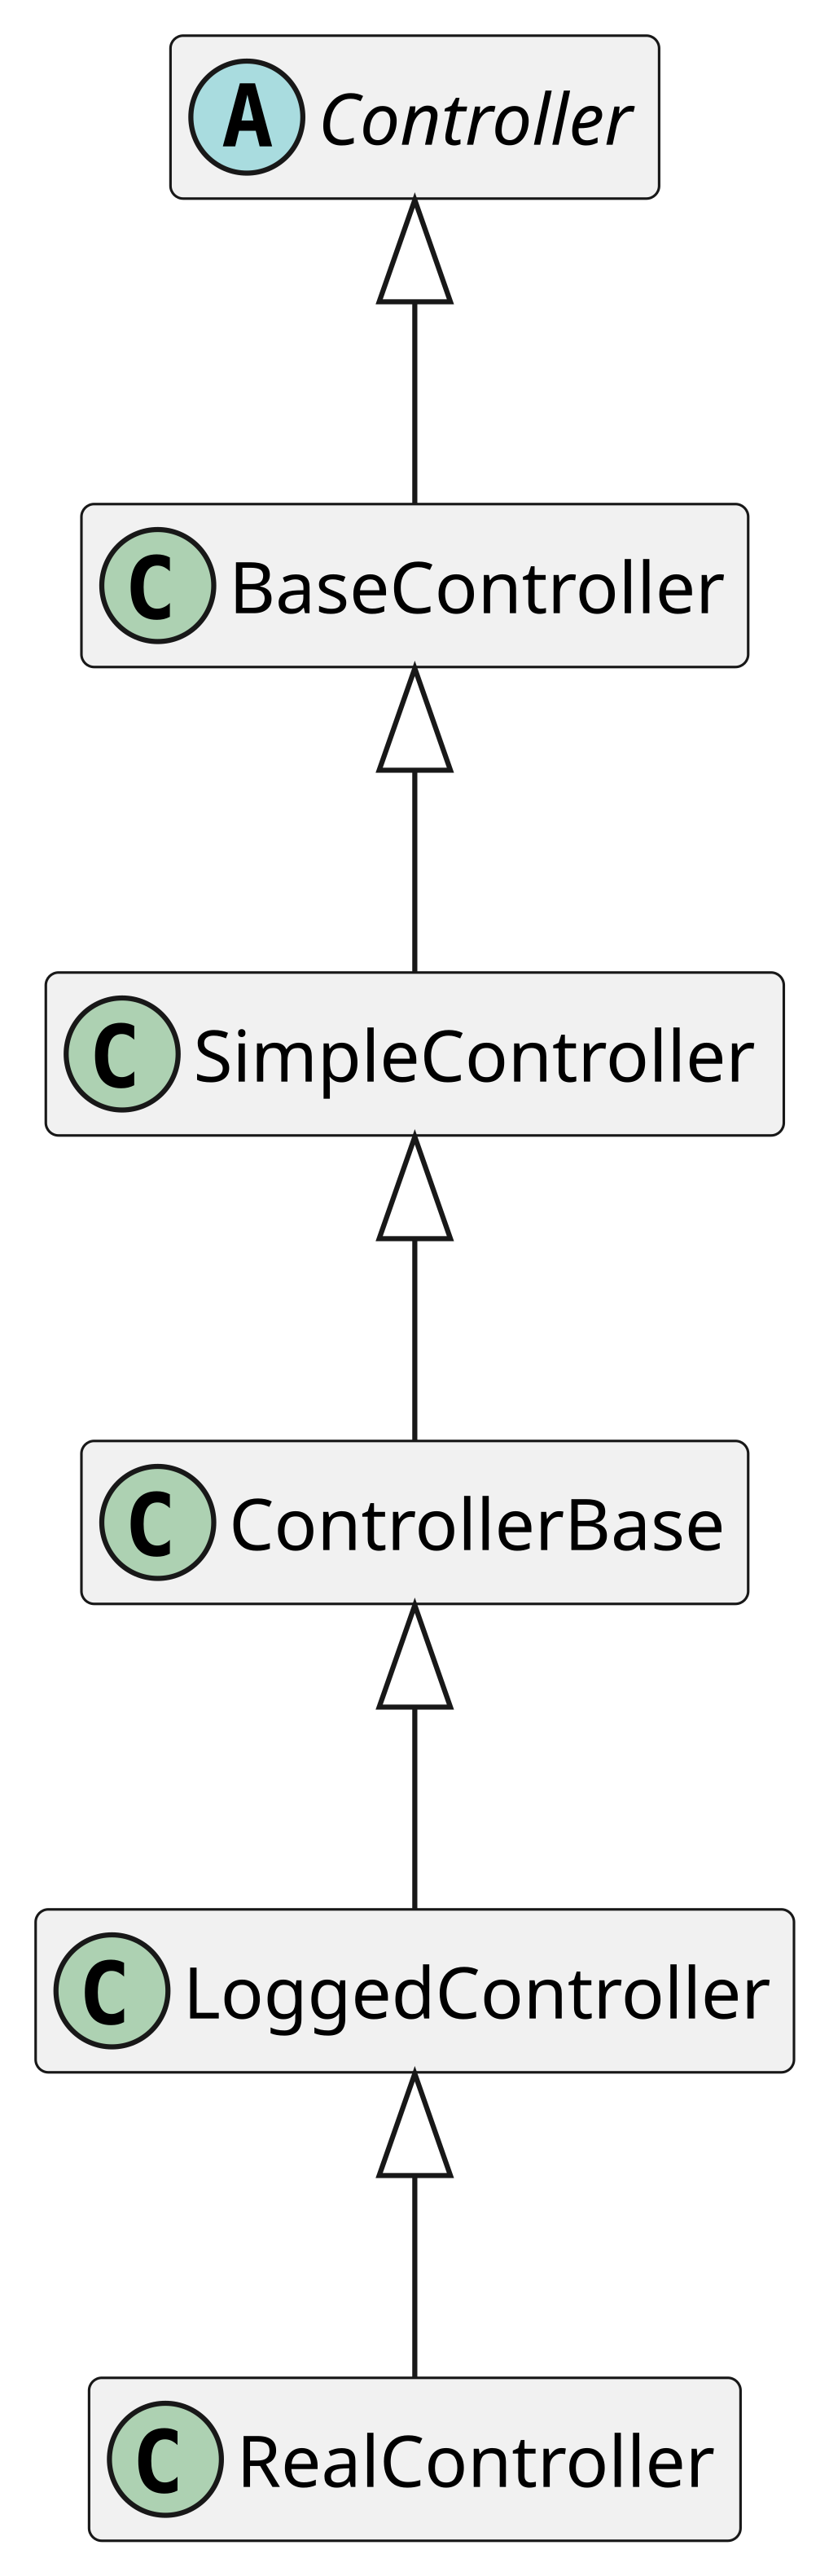
\includegraphics[height=.75\textheight]{src/session--composition-and-inheritance/resources/yo-yo-problem.png}
        \end{center}
    \end{minipage}\hfill
    \begin{minipage}{.80\textwidth}
        \begin{lstlisting}[numbers=none]
        <?php

        abstract class Controller {}

        class BaseController extends Controller {}

        class SimpleController extends BaseController {}

        class ControllerBase extends SimpleController {}

        class LoggedController extends ControllerBase {}

        class RealController extends LoggedController {}
        \end{lstlisting}
    \end{minipage}
\end{frame}

\begin{frame}
    \frametitle{OOP}
    \framesubtitle{Issues / Breaks encapsulation}

    \begin{itemize}
        \item Breaks encapsulation\pause
              \textcolor{ecgrey!50}{
              \\Inheritance creates dependency between child and parent.\pause
              \\When a class inherit another class, we include all methods and attributes from parent
              class and expose to the child class, therefore we break the encapsulation.\pause
              \\The child object can access all the methods in parent object and overwrite them.\pause
              \\That creates a tightly coupled relation between child and parent class,
              also against the idea of OOP, which is hide the complexity in the
              object and interact by interface.}
    \end{itemize}
\end{frame}

\begin{frame}
    \frametitle{OOP}
    \framesubtitle{Issues / Breaks encapsulation}

    \begin{itemize}
        \item Inheritance of unnecessary methods\pause
              \textcolor{ecgrey!50}{
              \\Inheritance makes a child class inherit all the methods
              and properties from parent class, even if it is not used or not needed,
              that creates more complexity than the child class needs to.}
    \end{itemize}
\end{frame}

\begin{frame}[fragile,c]
    \begin{center}
        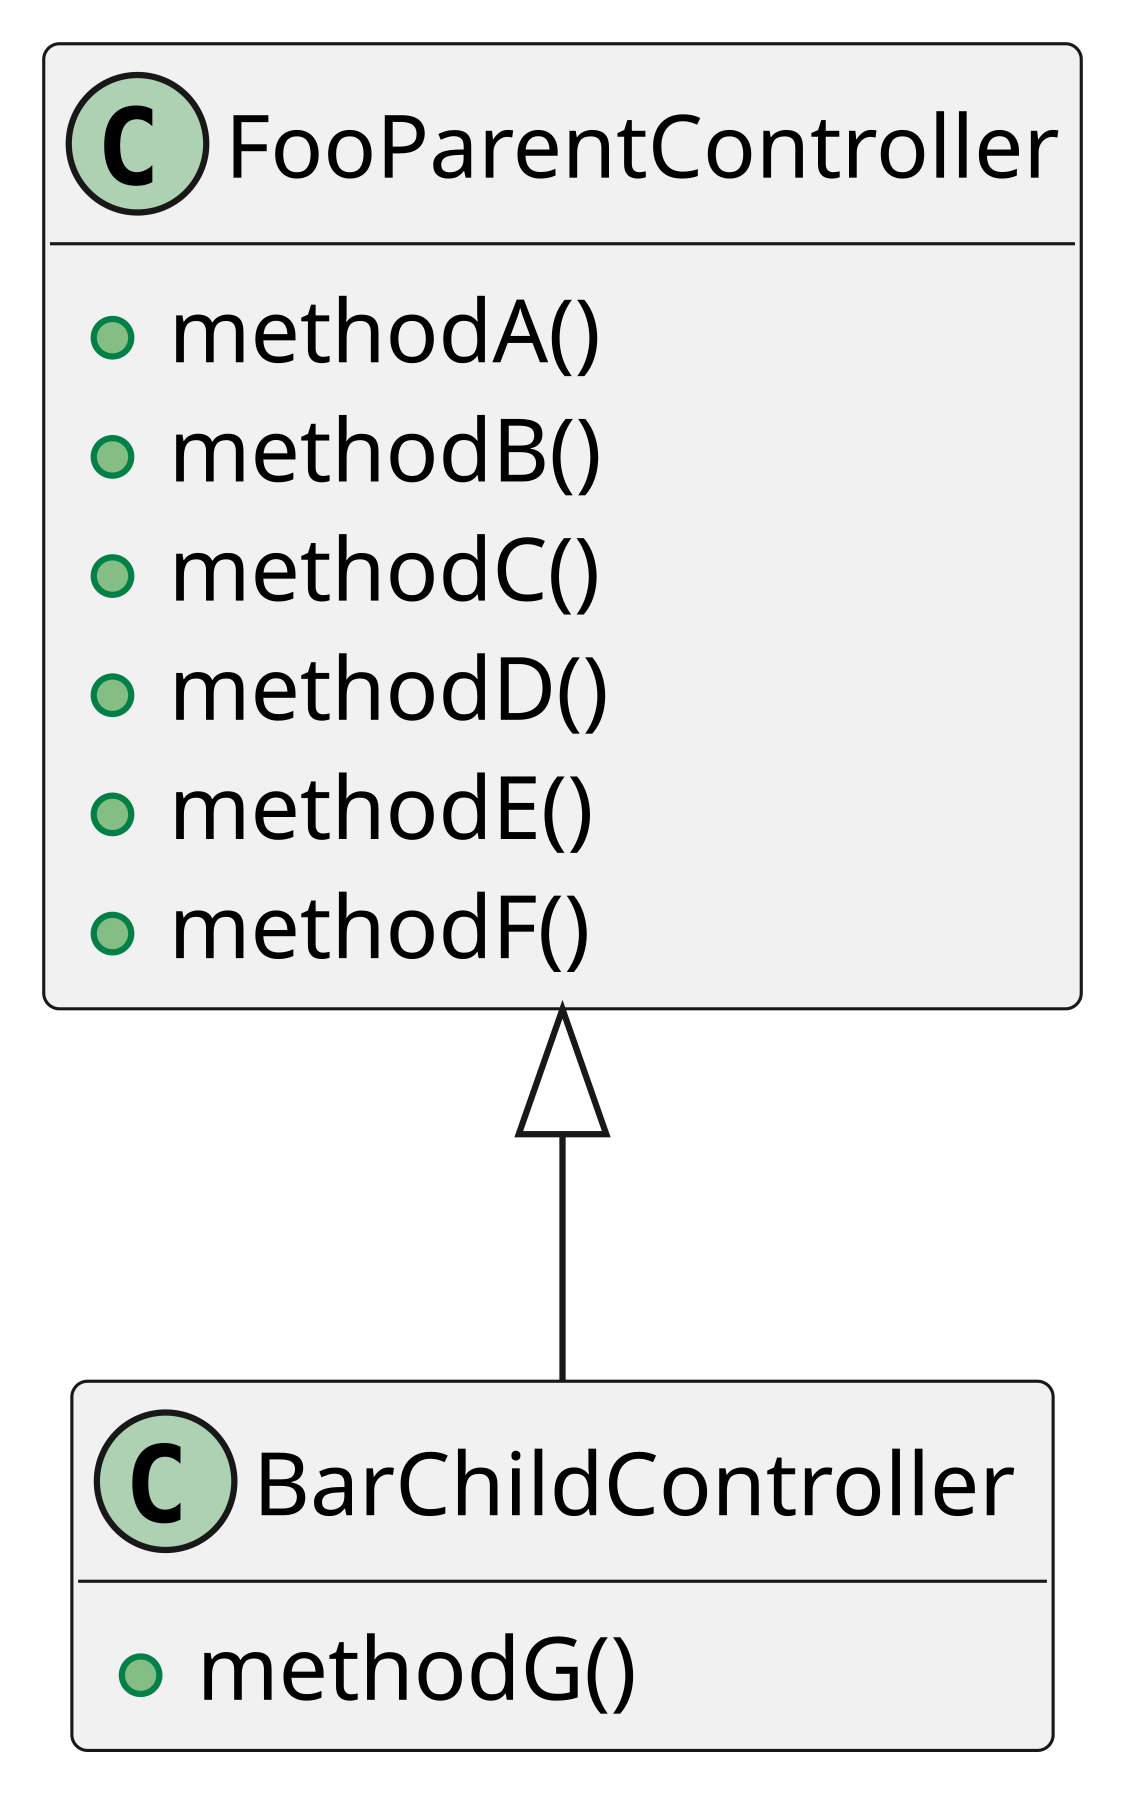
\includegraphics[height=\textheight]{src/session--composition-and-inheritance/resources/break-encapsulation.png}
    \end{center}
\end{frame}

\begin{frame}
    \frametitle{OOP}
    \framesubtitle{Issues}

    \begin{itemize}
        \item Flexibility\pause
              \\\textcolor{ecgrey!50}{A class can only inherit from one parent class.}
        \pause
        \item \texttt{Is-a} relation\pause
              \textcolor{ecgrey!50}{
              \\By extending a class, we also enforce an \texttt{is-a} relationship between
              parent and child, which sometimes does not reflect object’s real relationships.}
    \end{itemize}
\end{frame}

\begin{frame}[fragile,c]
    \frametitle{OOP}
    \framesubtitle{Issues / \texttt{is-a} relation}

    \begin{lstlisting}
    /**
     * Last-In-First-Out (LIFO) stack.
     */
    class Stack extends ArrayObject {
        /**
         * Push a value in the stack.
         */
        public function push(mixed $value): void
        {
            $this->append($value);
        }

        /**
         * Get and remove current stack value.
         */
        public function pop(): mixed
        {
            $arrayCopy = $this->getArrayCopy();
            $result = array_pop($arrayCopy);
            $this->exchangeArray($arrayCopy);

            return $result;
        }
    }
    \end{lstlisting}
\end{frame}

\begin{frame}
    \frametitle{OOP}
    \framesubtitle{Issues / \texttt{is-a} relation}

    \begin{itemize}
        \item Semantically, the statement "a \texttt{Stack} \texttt{is a} \texttt{ArrayObject}"
              is not true.\pause
              \textcolor{ecgrey!50}{
              \\\texttt{Stack} is not a proper subtype of \texttt{ArrayObject}.
              A stack is supposed to enforce \textit{Last-In-First-Out (LIFO)}, a constraint easily
              satisfied by the \texttt{Stack::push()} and \texttt{Stack::pop()} methods,
              but not enforced by the \texttt{ArrayObject}’s methods.}
        \pause
        \item Mechanically, inheriting from \texttt{ArrayObject} violates encapsulation.\pause
              \textcolor{ecgrey!50}{
              \\Using \texttt{ArrayObject} is an implementation choice that should be
              hidden from consumers.}
        \pause
        \item Finally, implementing a stack by inheriting from \texttt{ArrayObject} is
              a cross-domain relationship.\pause
              \textcolor{ecgrey!50}{
              \\\texttt{ArrayObject} is a randomly-accessible collection while a stack is
              a queuing concept.}
    \end{itemize}
\end{frame}

\begin{frame}[fragile,c]
    \begin{center}
        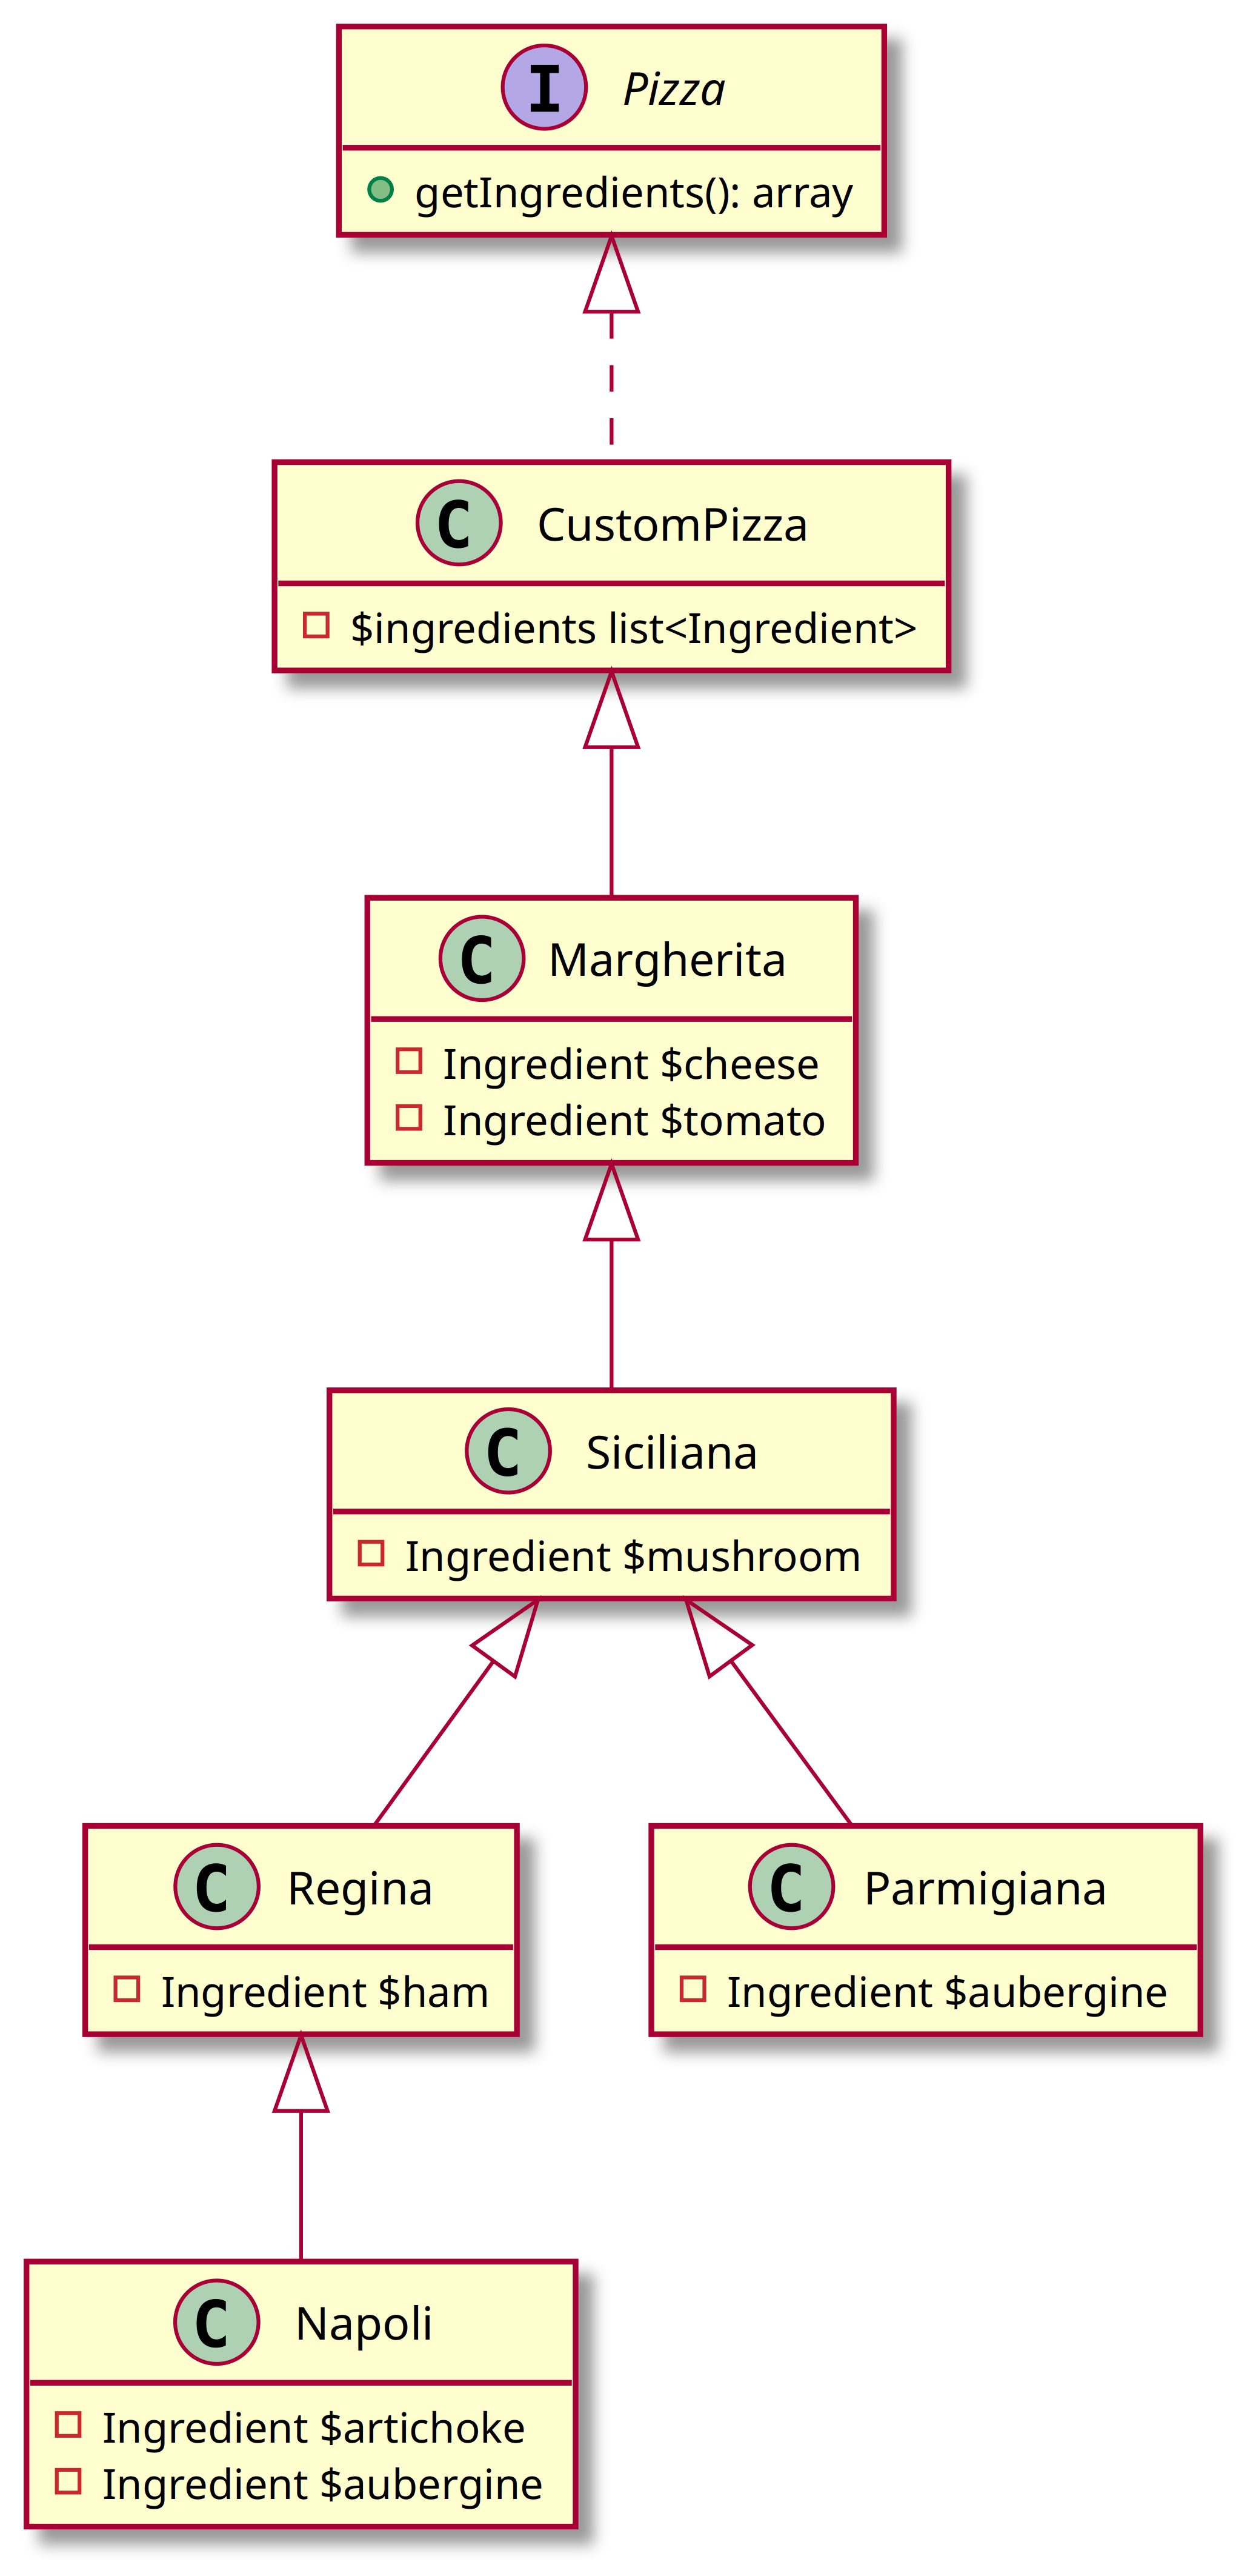
\includegraphics[height=\textheight]{src/session--composition-and-inheritance/resources/summary-oop-pizza.png}
    \end{center}
\end{frame}

\begin{frame}[fragile,c]
    \begin{lstlisting}
<?php

interface Ingredient {}

interface Pizza {
    public function getIngredients(): array;
}
    \end{lstlisting}
\end{frame}

\begin{frame}[fragile,c]
    \begin{lstlisting}
<?php

final class CustomPizza implements Pizza
{
    public function __construct(
        Ingredient ...$ingredients
    ) {}

    public function getIngredients(): array
    {
        return $this->ingredients;
    }
}
    \end{lstlisting}
\end{frame}

\begin{frame}[fragile,c]
    \begin{lstlisting}
<?php

class Margherita extends customPizza
{
    public function __construct(
        Ingredient $tomato,
        Ingredient $cheese
    ) {
        parent::__construct($tomato, $cheese);
    }

    public function getIngredients(): array
    {
        return parent::getIngredients();
    }
}
    \end{lstlisting}
\end{frame}

\begin{frame}[fragile,c]
    \begin{lstlisting}
<?php

class Siciliana extends Margherita
{
    public function __construct(
        Ingredient $tomato,
        Ingredient $cheese,
        private Ingredient $mushroom
    ) {
        parent::__construct($tomato, $cheese);
    }

    public function getIngredients(): array
    {
        return [...parent::getIngredients(), $this->mushroom];
    }
}
    \end{lstlisting}
\end{frame}

\begin{frame}[fragile,c]
    \begin{lstlisting}
<?php

class Regina extends Siciliana
{
    public function __construct(
        Ingredient $tomato,
        Ingredient $cheese,
        Ingredient $mushroom,
        private Ingredient $ham
    ) {
        parent::__construct($tomato, $cheese, $mushroom);
    }

    public function getIngredients(): array
    {
        return [...parent::getIngredients(), $this->ham];
    }
}
    \end{lstlisting}
\end{frame}

\begin{frame}[fragile,c]
    \begin{lstlisting}
<?php

class Parmigiana extends Siciliana
{
    public function __construct(
        Ingredient $tomato,
        Ingredient $cheese,
        Ingredient $mushroom,
        private Ingredient $aubergine
    ) {
        parent::__construct($tomato, $cheese, $mushroom);
    }

    public function getIngredients(): array
    {
        return [...parent::getIngredients(), $this->aubergine];
    }
}
    \end{lstlisting}
\end{frame}

\begin{frame}[fragile,c]
    \begin{lstlisting}
<?php

class Napoli extends Regina
{
    public function __construct(
        Ingredient $tomato,
        Ingredient $cheese,
        Ingredient $mushroom,
        Ingredient $ham,
        private Ingredient $aubergine,
        private Ingredient $artichoke
    ) {
        parent::__construct($tomato, $cheese, $mushroom, $ham);
    }

    public function getIngredients(): array
    {
        return [...parent::getIngredients(), $this->aubergine, $this->artichoke];
    }
}
    \end{lstlisting}
\end{frame}

\begin{frame}[fragile,c]
    \begin{lstlisting}
<?php

var_dump($margherita instanceof Pizza);       // true
var_dump($margherita instanceof $siciliana);  // true
var_dump($margherita instanceof $regina);     // true
var_dump($margherita instanceof $parmigiana); // true
var_dump($margherita instanceof $napoli);     // true
    \end{lstlisting}
\end{frame}

